\documentclass[11pt,a4paper,oneside]{article}
\usepackage[left=2cm,right=2cm,top=2cm,bottom=2cm]{geometry}
\usepackage[document]{ragged2e}
\usepackage[utf8]{inputenc}
\usepackage{amsmath}
\usepackage{amsfonts}
\usepackage{amssymb}
\usepackage{graphicx}
\usepackage{xcolor}
\usepackage{subfig}
\usepackage[output-decimal-marker={.}]{siunitx}
\usepackage{wrapfig}
\usepackage{lipsum}
\usepackage[toc]{appendix}
\usepackage{eso-pic}
\usepackage{hyperref}
\usepackage{siunitx}
\newcommand{\commento}[1]{{\color{purple}{#1}}\vspace{10pt}}

\title{%
 \vspace{-2.0cm}
 Exploring Onset Finding Algorithms: A Monte Carlo \\ Simulation For  Hyperfine Splitting Measurement of Anti-Hydrogen
}

\date{\vspace{-5ex}}
\author{Adriano, Simone,Germano }
\begin{document}

\AddToShipoutPicture*
    {\put(530,775){
\includegraphics[width = 0.09\textwidth]{logo/ALPHA_Logo.jpg}}}

\maketitle


\paragraph{Introduction}

In this report we present a simple Monte Carlo simulation developed within the context of ALPHA-2 Hyperfine Splitting measurement. The objective of this study is to assess the statistical uncertainty and bias of the algorithm utilized in 2017 analysis when applied to the new arrangement of data collected in 2023. In addition to this, different algorithms have been tested, as alternatives of the algorithm used in the previous analysis.

The Hyperfine Splitting Measurement consists on the determination of the $\Delta f$ frequency transitions between $c \rightarrow b$ and $ d \rightarrow a$ states of anti-hydrogen. This measure is carried out in ALPHA-2, where the anti-hydrogen is irradiated with the light produced by a laser with variable frequency. Due to the transitions induced by the light, a certain amount of anti-hydrogen is released from the trap and annihilates. The counts of anti-hydrogen annihilation per frequency constitutes the experimental \textit{line-shape}. During the experiment, the \textit{line-shape} of the $c \rightarrow b$ and $ d \rightarrow a$ transitions are measured. The Hyperfine Splitting is determined by the frequency interval between the two \textit{line-shapes}, which is estimated taking the difference of the frequency onset of the two \textit{line-shapes}. This study is done using \textit{ROOT} and \textit{RDataFrame} framework. All the software used for the simulation can be found here: {\color{blue}{\url{https://gitlab.cern.ch/alpha-italy/psr-toymc}}}

\section{Purpose of the simulation}

The aim of the experiment is to measure the c to b and d to a transitions, extract the \textbf{onset} of each transition and compare the two value to measure the hyperfine splitting on anti-hydrogen. The core of the simulation is to reproduce the experimental procedures to obtained the hyperfine splitting of anti-hydrogen from the series of run collected in 2023 at ALPHA-2 apparatus. A first important consideration is that the simulation does not account atomic physics or dynamical simulation of trapped anti-hydrogen in order to reproduce the shape of anti-hydrogen transition. This type of study is not pertinent to the present work, and it is delegated to other members of the collaboration.
In fact, the simulation focuses on the experimental procedure to extract the onsets frequency from the data, seeking to replicate those experimental effects that influence the measurement and contribute to both statistical and systematic error.
In this context, the simulation begins by assuming a specific form of transition. The model used for the c to b and d to a transitions has been derived with a maximum likelihood fit the data of high statistic \texttt{run 69373}, (\url{https://alphacpc05.cern.ch/elog/DataLog/100293}). The function used is a truncated Cruiff function, which is a modified version of a gaussian which accounts for the possibility of having asymmetric tails.

\begin{equation} \label{eq:Cruiff}
    \begin{cases}
      baseline \qquad & x < onset\\
      N \cdot \exp \left( \dfrac{ -( x - x_{0})^2}{2 \sigma_{0}^{2} + k_{0}(x - x_{0})^2} \right) + baseline \qquad & onset <= x < x_{0} \\
      N \cdot \exp \left( \dfrac{ -( x - x_{0})^2}{ 2 \sigma_{1}^{2} + k_{1}(x - x_{0})^2} \right) + baseline \qquad & x > x_{0}
    \end{cases}\,.
\end{equation} 

We point out that this model is a rough estimation of the true line-shape of the transition. We expect the shape of the transition to be influenced by the power of the microwave laser used to induce it, and the model used to generate the data is only a rough approximation of how the real data look like. The function has six free parameters, and the value of the onset was fixed at $\SI{175}{ \kilo \hertz}$.

\begin{figure}[!hbtp]
\centering
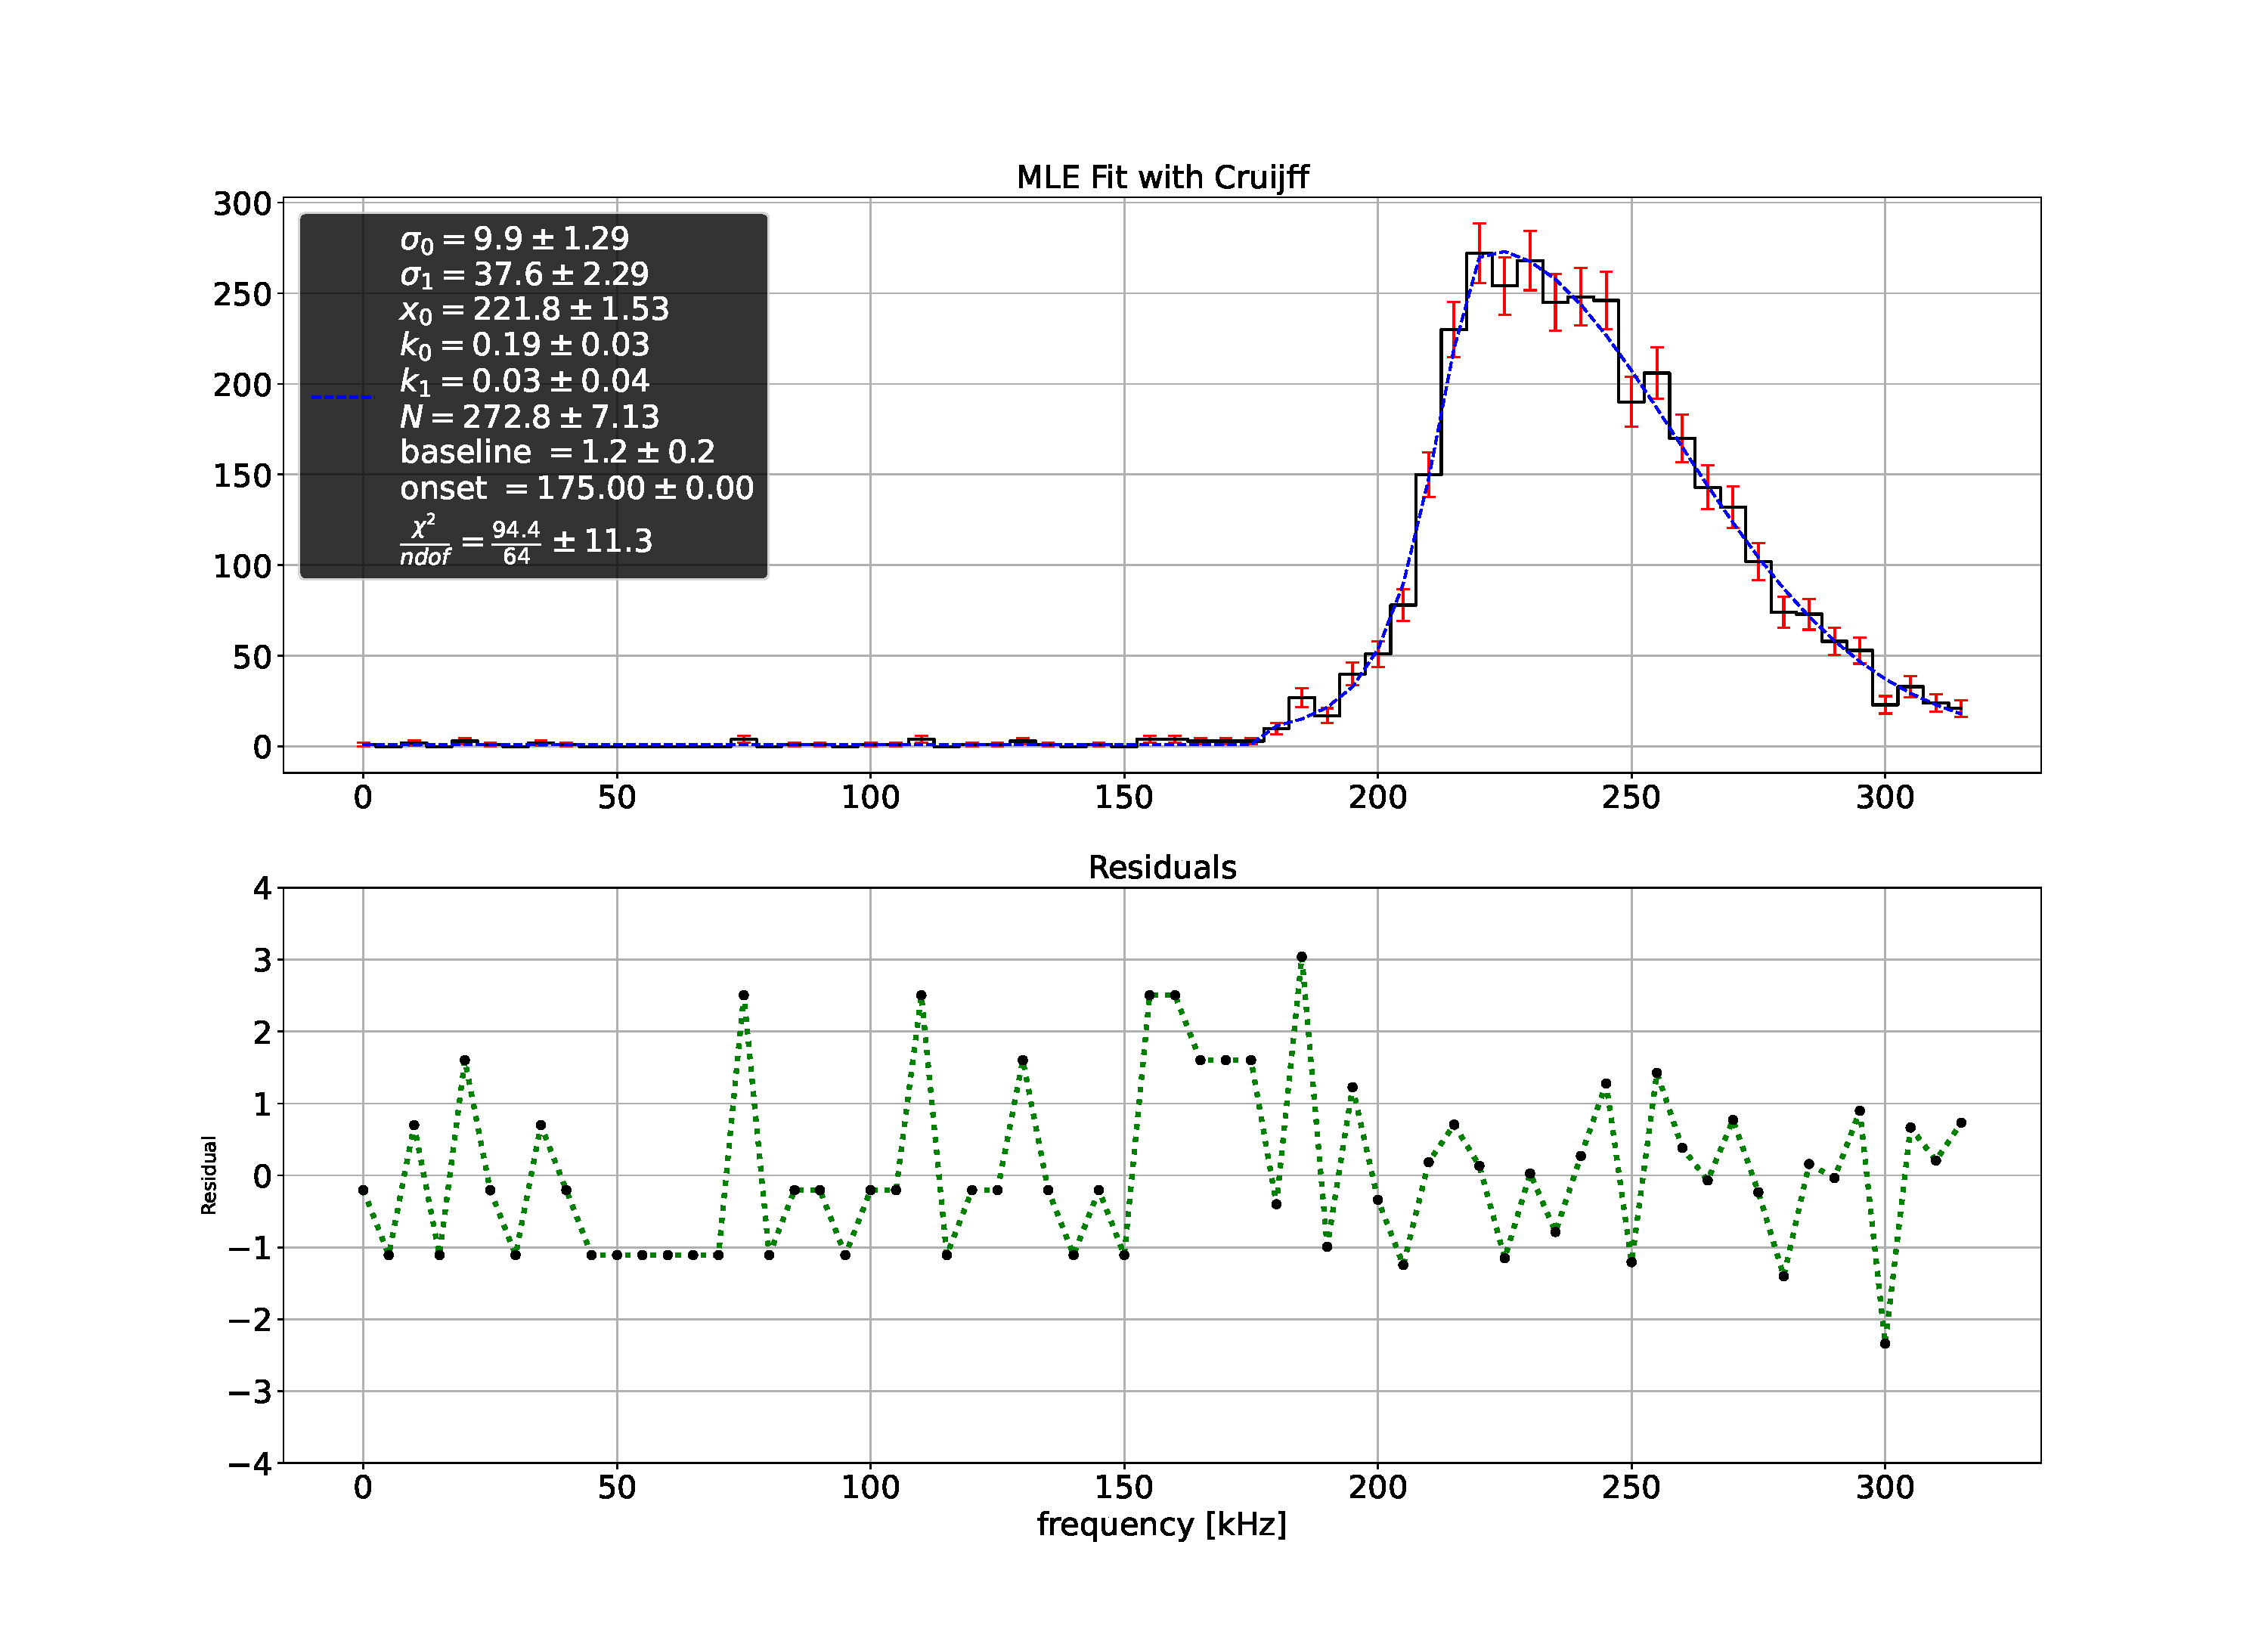
\includegraphics[width=1\textwidth]{cruijffFit.pdf}
\end{figure}

The model describes so far is not the only model that we have used in to fit the data. We have also considered the same model with a quadratic and linear rise. This different rise shape are included in the simulation, which are useful to study the effects of the different rise asymmetries on the hyperfine splitting extraction, in order to study the systematic error of the measurement. 

\subsection{Discretization of the Line-Shape}
\commento{Need to be expanded, include more details about how the data are generated}

The starting point of the simulation involves constructing a model that can adequately describe the two transitions to be measured in the experiment, and that can be used to generate the data. In the simulation, we have used the function defined in \ref{eq:Cruiff}, with a proper normalization procedure, which is described in this section. 

From the function fitted to the high statistic data, we have removed the baseline, because the background events (which encompass both residual gas and cosmic) are generated separately and later combined together with the annihilation coming from the two transitions. To retrieve the correct normalization of the \textit{pdf}, the function is discretized in a series of $50$ equally spaced points ($y_{i}$), with a frequency step given by the scenario to be reproduced. The $y_{i}$ are then normalized so that:

\begin{equation}
\sum_{i = 0}^{N = 50} y_{i} = 1
\end{equation}

We use the model with this constrain to generate the annihilation count for each frequency step. The counts per each frequency follows a poisson distribution with a mean given by

\begin{equation*}
y_{i} \, \epsilon \, N_{stack} N_{\overline{H}}  
\end{equation*}

to scale the model to the statistic used in the experiment ( $\epsilon$ is the efficiency, and $N_{stack}$ and $N_{\overline{H}}$ the number of stack and anti-hydrogen per stack).The routine for generating events is managed by ROOT, specifying the \textit{Extended()} options to introduce the poisson fluctuation in the number of counts.  

We want to highlight that in a real dataset, the length of the frequency sweep (aka, the number of frequencies measured) is less then the series of $50$ points used in the discretization. For the events belonging to frequencies that falls out of the sweep, they are marked with clearing flag, so that they can be properly handled in the analysis of the simulation results.

\begin{figure}[!hbtp]
\centering
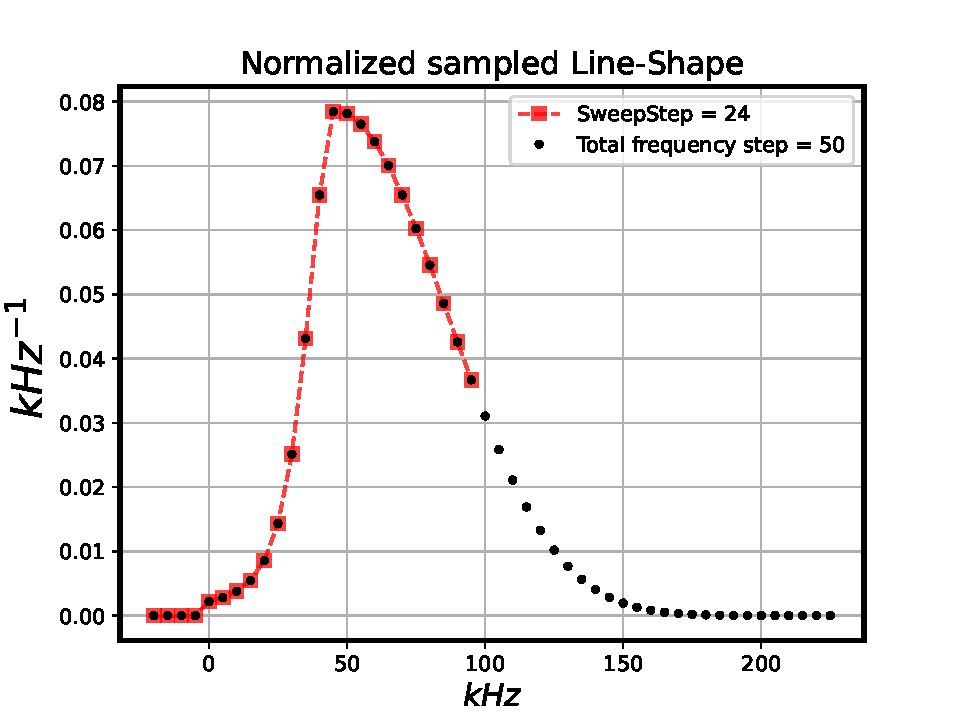
\includegraphics[width=0.85\textwidth]{Normalized.pdf}
\caption{Example of normalized Line-Shape, sampled with a frequency step of $\SI{5}{\kilo \hertz}$ with 50 frequency step. The red square dot represents the fraction corresponding to a sweep of $24$ steps The starting point is the initial values of the sweep, and it supposed to fluctuate based on how the operator set the initial frequency.}
\end{figure}

\begin{figure}[!hbtp]
\centering
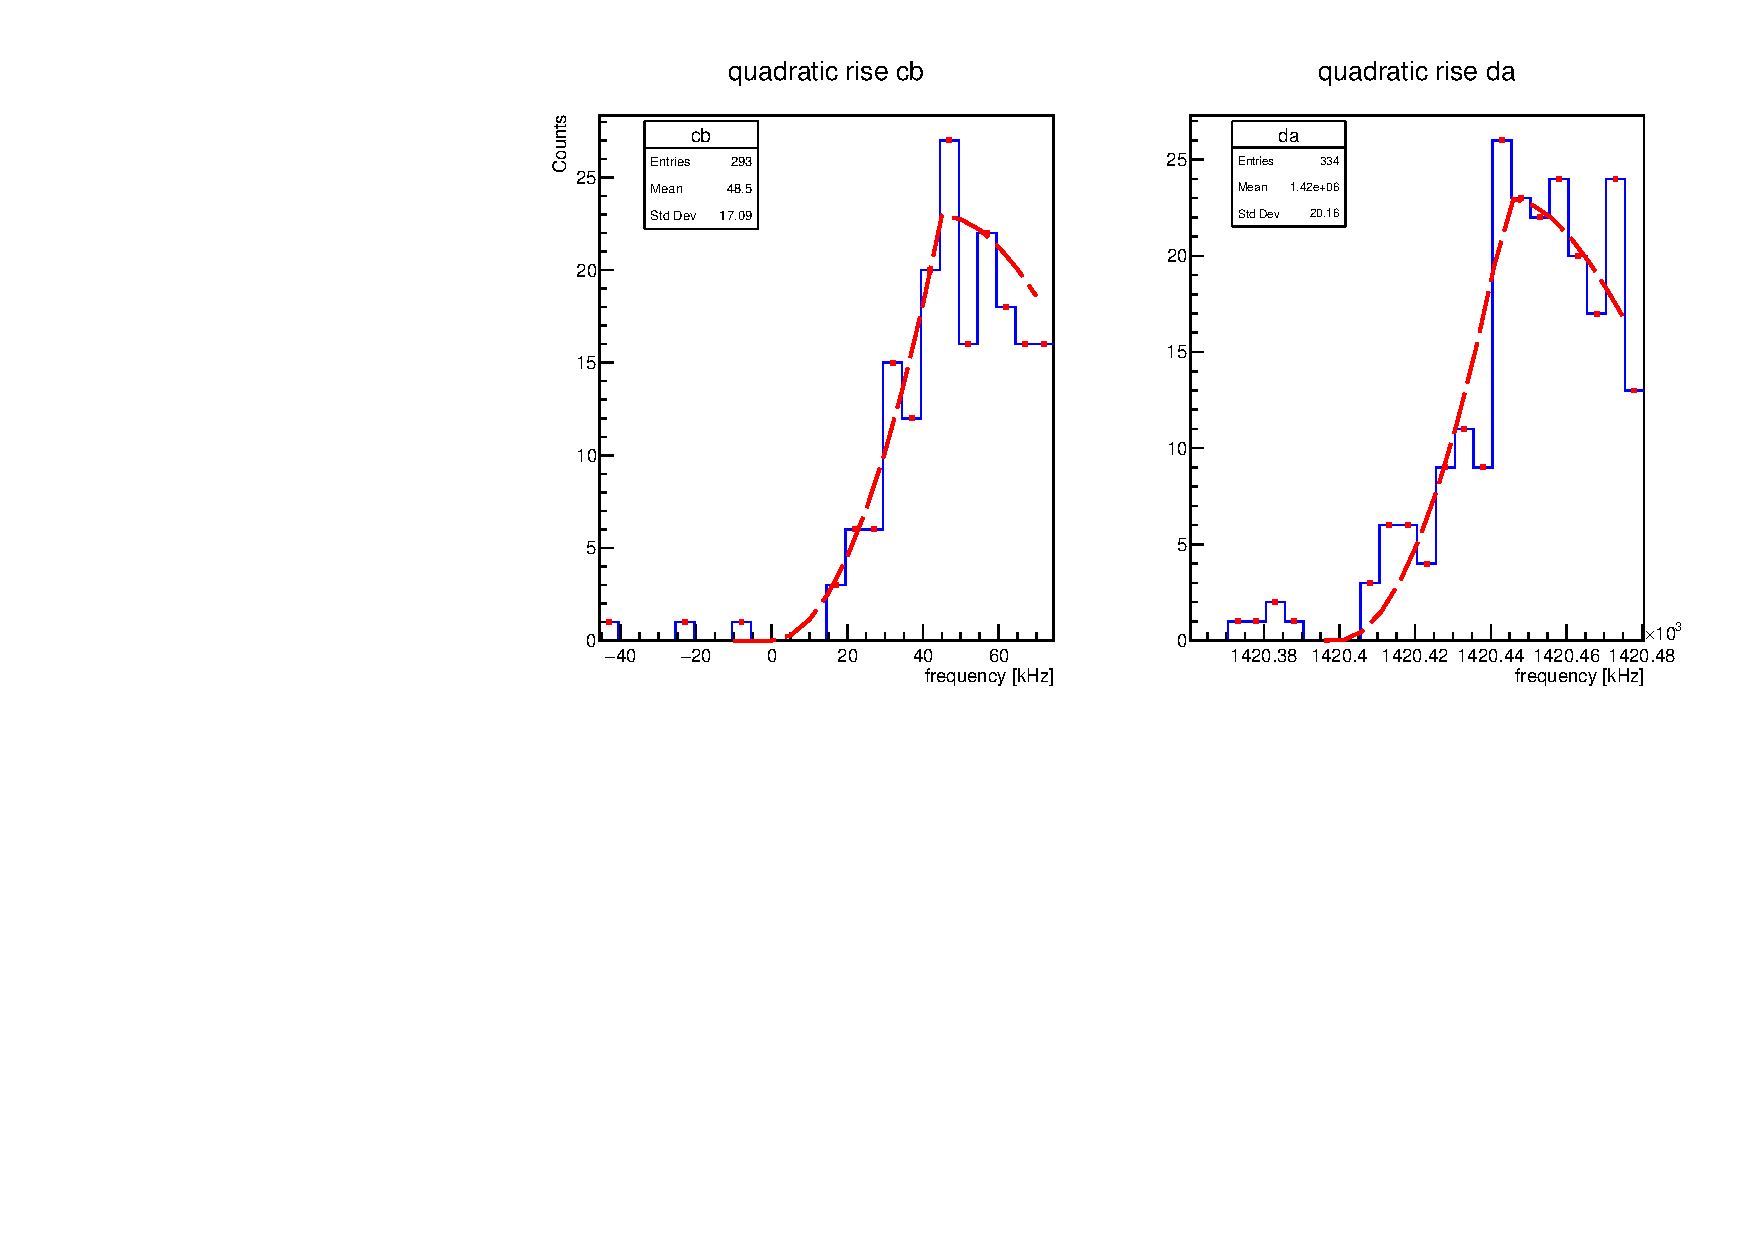
\includegraphics[width = 0.9\textwidth]{examplePasscut.pdf}
\caption{Example of line-shape generation, where each transition was generated with a statistic of $N_{\overline{H}}] \simeq 300 $}
\label{fig:ExampleGen}
\end{figure}

Regarding the background events, We made very simple assumptions, considering that the events were uniformly distributed in frequency. In figure \ref{fig:ExampleGen} we report two example of generated transition

\subsection{Radius Variable}

\commento{complete, are we planning to do something with radius? For instance a likelihood ratio to cut out background.}

An anti-hydrogen annihilation can occur in two different modes: the first one is due to the excitation of the micro wave field, which drive out the $\overline{H}$ into an un-trappable state. The $\overline{H}$ is then no more confined by the magnetic field of the trap, and annihilates on the trap wall. The second mode are made by those annihilations resulting from residual gas inside the magnetic trap. It can depend on the goodness of the vacuum or/and the temperature of the electrodes, which are heated during the experiment. Ultimately, one must consider also the cosmic background, which is mainly constituted by muons which are erroneously classified as $\overline{H}$ events. 

These different annihilation process are characterized by different radius distribution of the reconstructed vertex. The \textit{pdf} of the radius distribution are shown in figure \ref{fig:RadiusDistributions}

\begin{figure}[!hbtp]
\centering
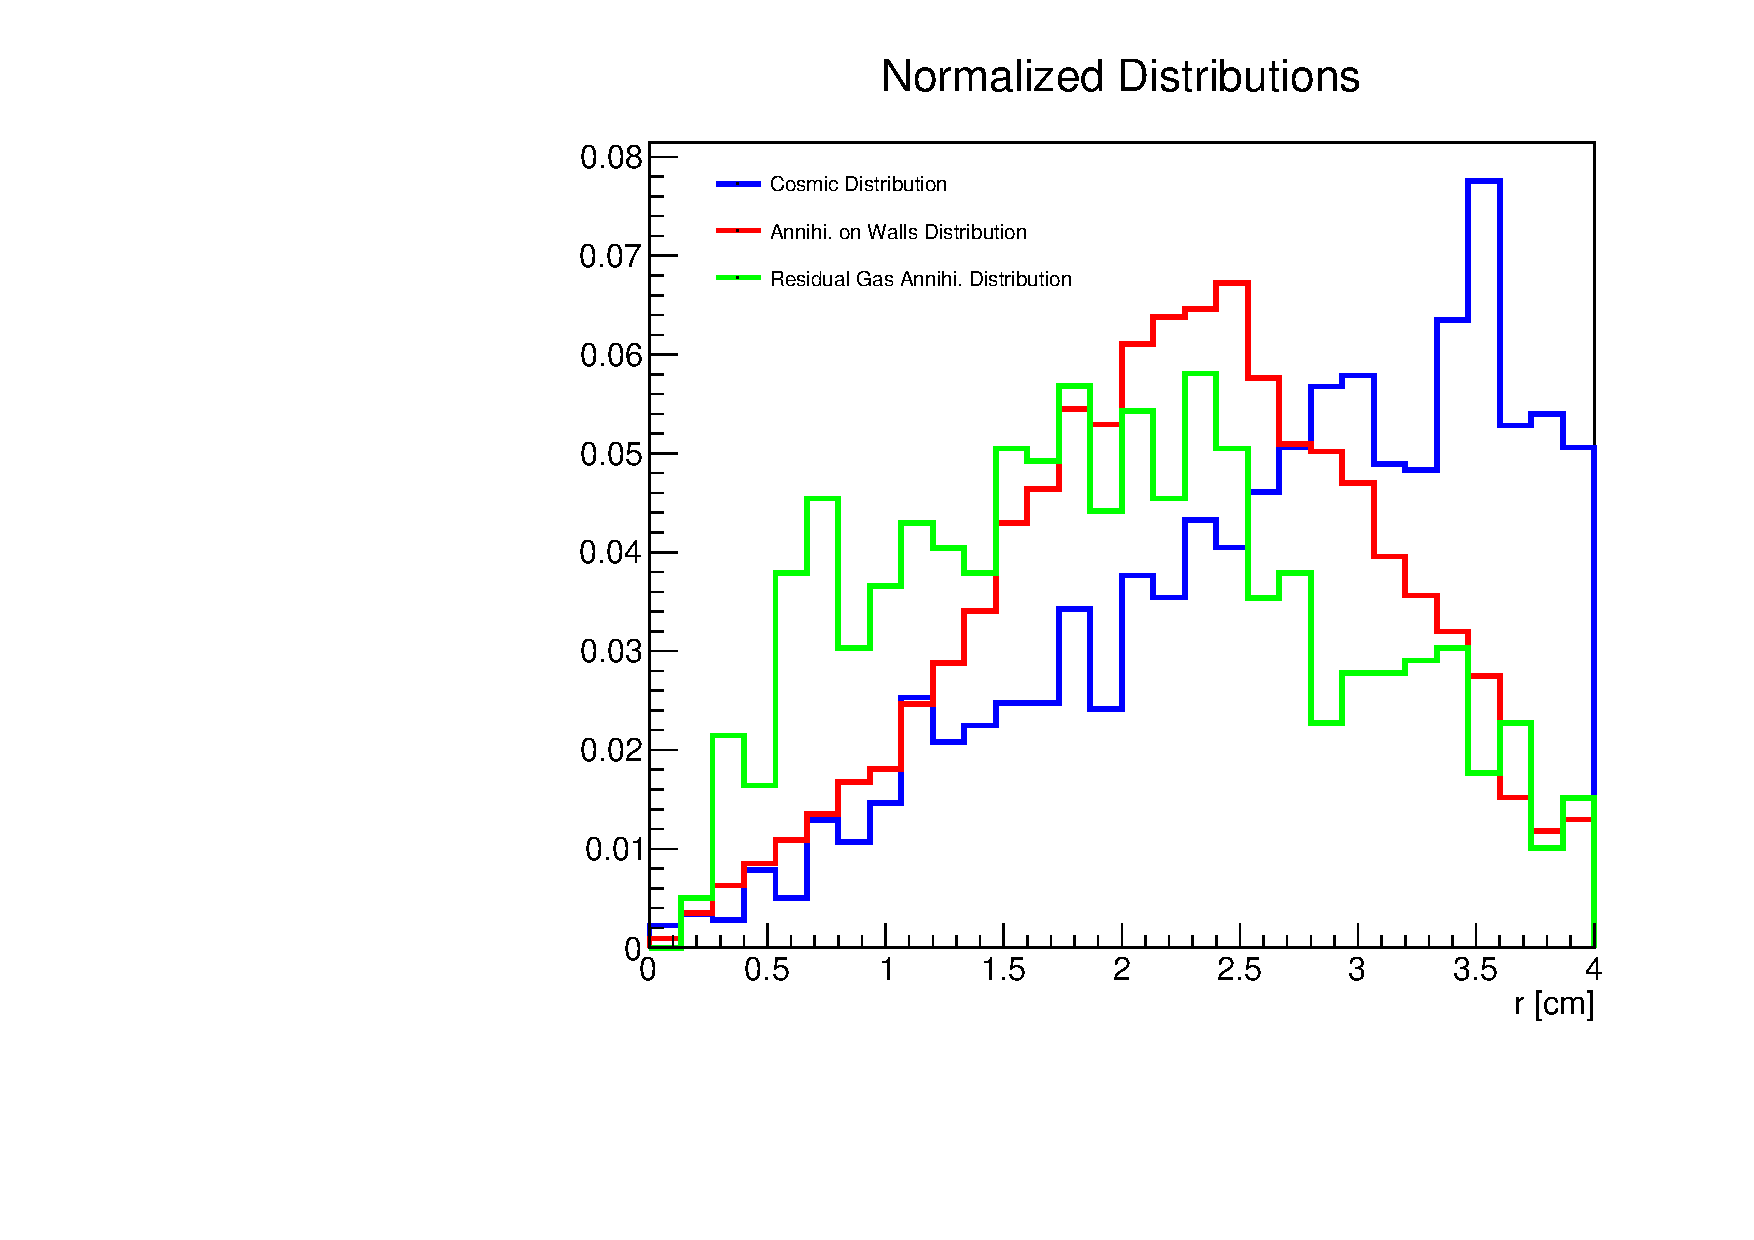
\includegraphics[width = 0.75\textwidth]{PdfTogether.pdf}
\caption{Radius distribution and radial density distribution for the three different events that can occur in the alpha-2 magnetic trap.}
\label{fig:RadiusDistributions}
\end{figure}

The PDFs shown in figure were studied individually using datasets where only one type of annihilation was present at a time. For the cosmic distribution (highlighted in blue), we have used a series of run with no anti-hydrogen in the trap. For the annihilation on trap walls, we have used data regarding the mixing phase, were in a interval of $\SI{2}{\second}$ the $\overline{p}$ annihilates on trap walls. The Residual gas distribution is obtained for $\overline{H}$ in the trap wall that were illuminated by off-resonant micro-wave light. The micro-wave light heats up the electrodes and consequently also the residual gas in the trap, that increases the annihilation due to residual gas \footnote{Chiedere a Simone, non ricordo bene se fosse esattamente così}.

In the simulation, for each annihilation or cosmic background, a vertex radius following the curves in figure \ref{fig:RadiusDistributions} is generated.

\section{Brief description of the experiment}

In this section we describe the experimental procedure that was followed out during the data taking of 2023. 
The acquired data comprises a series of runs where a single measurement of the "cb" transition, followed by "da" transition measurement, is carried out and repeated a certain number of times. Each individual "cb" and "da" named \textit{repetition}. A collection of \textit{repetitions} represent a dataset, that can be used to extract the value of the hyperfine splitting.  During the measurement, the magnetic field of the superconducting magnets is drifting, and this implies that the frequencies at which the transitions occur shift over time. During the experimental campaign, the windows at which the transitions are sampled are adjusted to track the shifts caused by the magnetic field, which linearly depend on time.
The value of the magnetic field drift are measured with the ECR, and are approximately $ \SI{-72}{\kilo \hertz \second\tothe{-1}} \pm \SI{2}{\kilo \hertz \second\tothe{-1}}$, (see figure \ref{fig:ECR}).

\begin{figure}[!h]
\centering
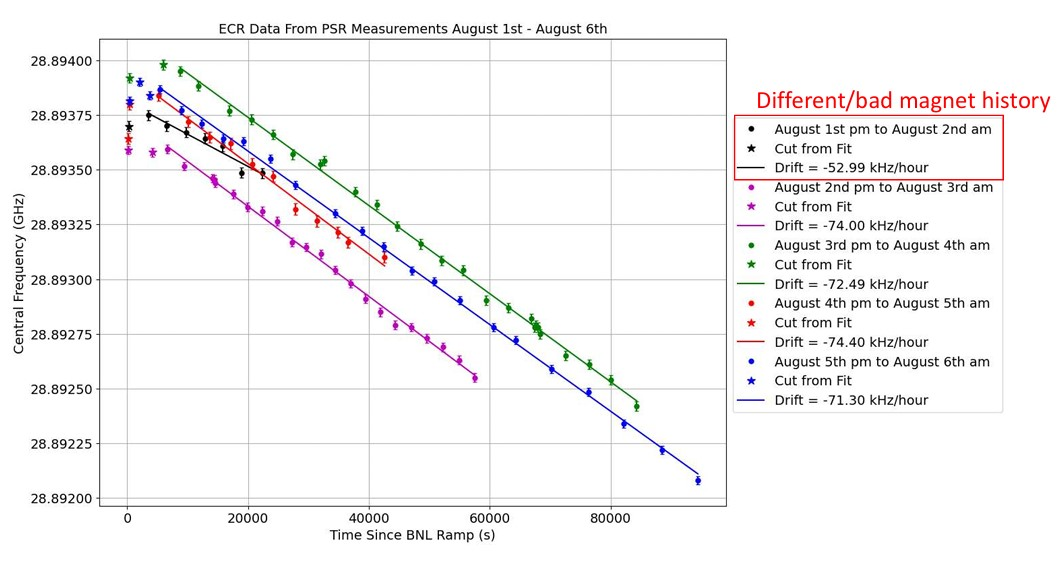
\includegraphics[width = \textwidth]{ECR.jpg}
\caption{ECR measurement for the different series of data.}
\label{fig:ECR}
\end{figure}

Because of the magnetic drift, the direct measurement of the frequency interval between the \textit{cb} and \textit{da} transitions does not depends only on the values of the hyperfine splitting of anti-hydrogen. Calling the starting point of the cb and da transitions as $onset_{cb}$ and $onset_{da}$, we have that:

\begin{align*}
onset_{cb}(t + \delta t_{1}) &= onset_{cb} (t) + B_{drift} \cdot \delta t_{1} \\
onset_{da}(t + \delta t_{2}) &= onset_{da} (t) + B_{drift} \cdot \delta t_{2}
\end{align*}

To visualize how the transition are drifted, we show in figure \ref{fig:MovingOnset} 5 simulated cb transitions, which occur at subsequent times. Since the measurement of the transitions 'da' and 'cb' cannot occur simultaneously, but take place at successive moments, namely $\Delta t = \delta t_{2} - \delta t_{1}$, we conclude that the difference between the two frequencies is given by:

\begin{equation} \label{eq:hfsmes}
onset_{da} - onset_{cb} = hfs + B_{drift} \cdot \delta t
\end{equation}


In this simplified picture, where we assumed to determine with $100 \%$ precision and accuracy the transition starting frequency, The measurement can only be performed with knowledge, whether previous or not, of the drift of the magnetic field.

\begin{figure}[!h]
\centering
\textbf{CB TRANSITIONS} \\
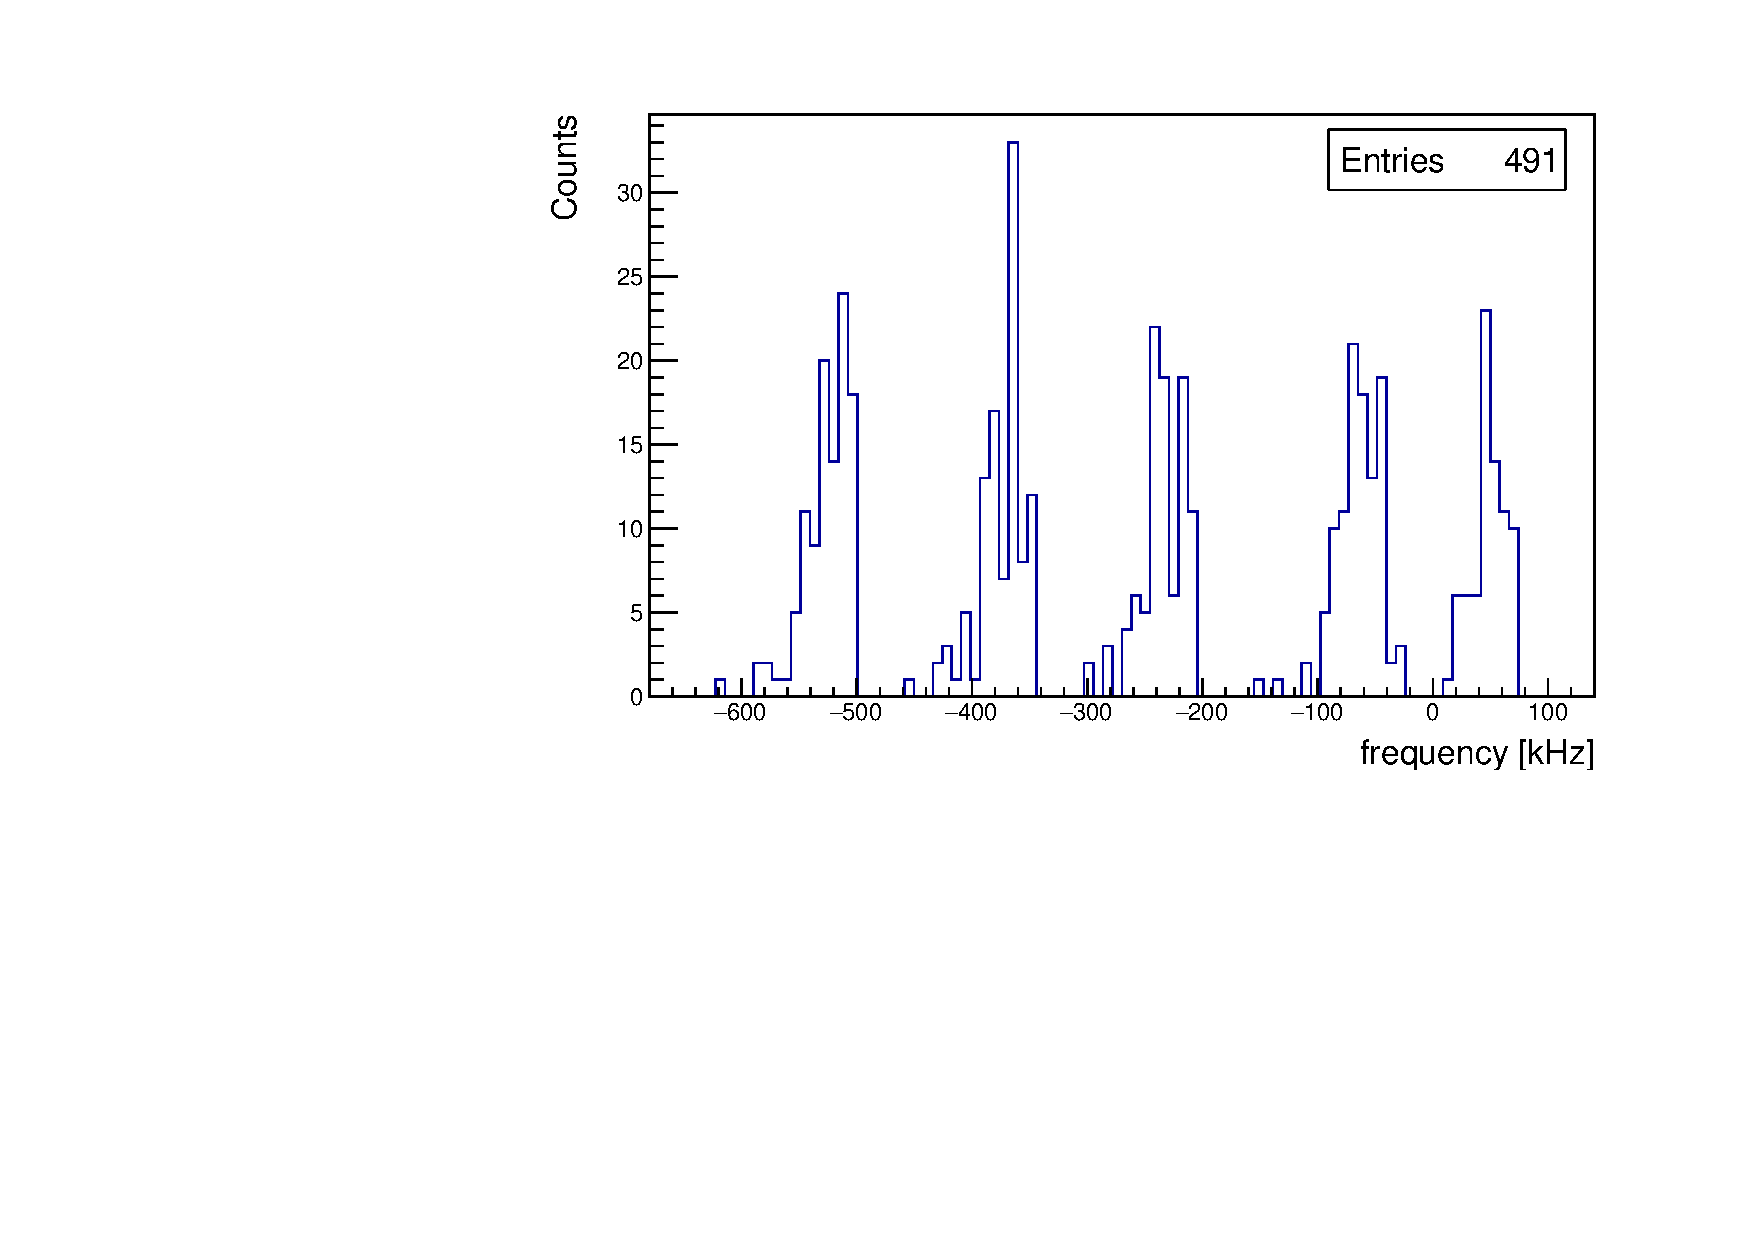
\includegraphics[width = 1\textwidth]{seriesoftransitions.pdf}
\caption[cb repetitions]{Simulated serie of cb transitions. The first transition on the right correspond to the first repetition. Since the magnetic field drift is negative, the next transition will are progressively shifted to the left.}
\label{fig:MovingOnset}
\end{figure}

\newpage
\subsection{List Of Random}
\commento{spiegare in dettaglio le motivazioni/come è stato implementato ogni random presente nella simulazione, e qualitativamente che effetto produce sui dati}

The objectives of our ongoing simulation we are developing aims to replicate the most significant aspects present in the measurement and investigate how this affects the experiment's outcome. Some of these effects are well understood and can be studied precisely. For others, quantitative estimates are unavailable, so reasonable values are employed in the simulation to approximate experimental reality.

This effects could increase the statistical uncertainty of the measurements or/and could be responsible for the presence of systematic effects for the result extraction. We give here a list of them with a brief explanation.

\begin{center}
\textit{List of randoms}
\end{center}

\begin{itemize}
\item $\Delta f_{start}$ frequency start: it represent the initial frequency that is set by the operator. It is uniformly distributed.   
\item $\sigma_{Bdrift}$ uncertainty estimation. The estimation of the $B_{drift}$ is used by the operator to set the starting point of the following repetition, in order to track the onset that are moving due to the change of the magnetic field. This value is generated from a normal distribution $N(\mu, \sigma)$, with $\mu = B_{drift}$ and $\sigma = \sigma_{Bdrift}$
\item $\delta t_{jitt}$ time jitter effects: this value is introduce to simulate a delay/advance in the beginning of the sweep compared to the value calculated considering the shift of the onsets due to the magnetic field
\item $\Delta t_{rep}$ time between repetitions: between one repetition and the next one some time passes for staking new anti-hydrogen in alpha2. The value is generated uniformly between 1 hour and half and two hour and half.
\item $N_{\overline{H}}$ number of anti hydrogen. This value is poisson distributed with a mean equal to $N_{\overline{H}}$
\item $\delta_{MC}$, which modifies the value of hyper-splitting of anti-hydrogen. It is used to study possible if and how effectively the experiment measures variations of the value of the hyperfine splitting (whose default value is assumed to be equal to that of hydrogen). The hyperfine splitting is modified such that $\overline{hfs} = hfs + \delta_{MC} $ where $\delta_{MC}$ is uniform distributed.
\item $\mu_{cosmic}$ cosmic background events. It one of the terms which contributed to the background of the experiment. It is generated flat for each frequency, following poissonian statistic. In the simulation is fixed to the expected value for PASSCUT, or changed accordingly to the MVA working point.
\item $\mu_{gas}$ residual gas annihilation rate. This is a component of the experimental background, which add up to the cosmic background. It is a possible source of systematic effects, since they have different for the two transitions. As for cosmic background, they follow a poissonian statistic and are generated flat in frequency.
\end{itemize}



\begin{figure}[!hbtp]
\centering
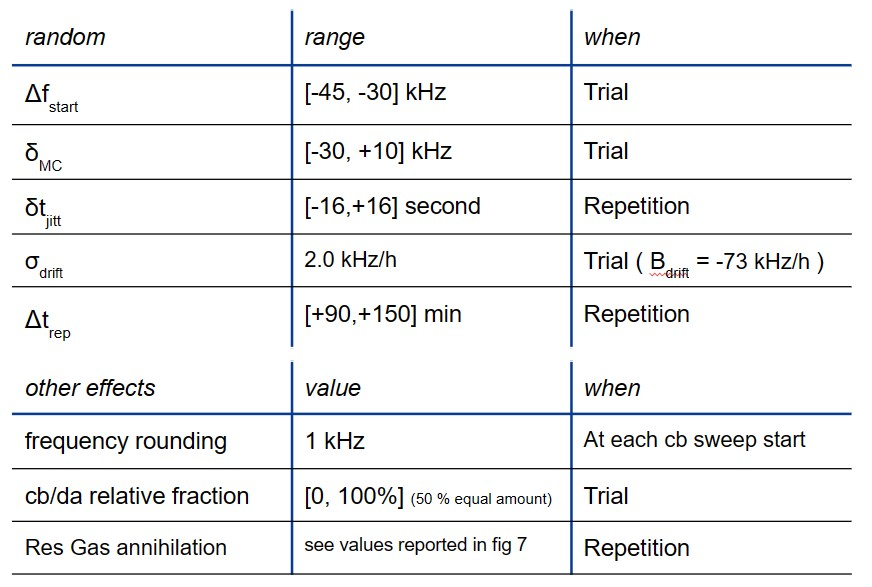
\includegraphics[width = 0.85\textwidth]{Screenshot 2024-04-21 173735.jpg}
\caption{ Set of parameters together with their values used in the simulation.}
\end{figure}

The values listed above are not the only parameters of the simulation, however they represent the set of parameters associated with a random generation. Other important parameters, related to the experimental configuration, are listed below, with a brief description.

\begin{center}
\textit{List of parameters}
\commento{\\ aggiungere breve spiegazione ad ognuno di essi, per ora sono solo elencati.}
\end{center}

\begin{itemize}
\item Number of repetitions
\item $B_{drift}$ value
\item frequency step
\item time step
\item Clearing steps
\item Sweep steps
\item rise length 
\item frequency rounding
\item type of rise ("quadratic", "linear", "Cruijff")
\item Parameters of the analytic models used to fit the high statistic run.
\item population asymmetry between c and d states.
\end{itemize}

There are also other parameters which a related to systematic effects which can occur in the measurement. The most important are: 

\begin{itemize}
\item population asymmetry between c and d states.
\item type of rise ("quadratic", "linear", "Cruijff")
\item rate of gas annihilation (which might be different for cb or da transition)
\end{itemize}

We will discuss their effects in a separate section. We have created a schematic overview to illustrate where and how all these effects come into play within the simulation, depicted in figure \ref{fig:AschemeRandom}

\begin{figure}[!hbtp]
\centering
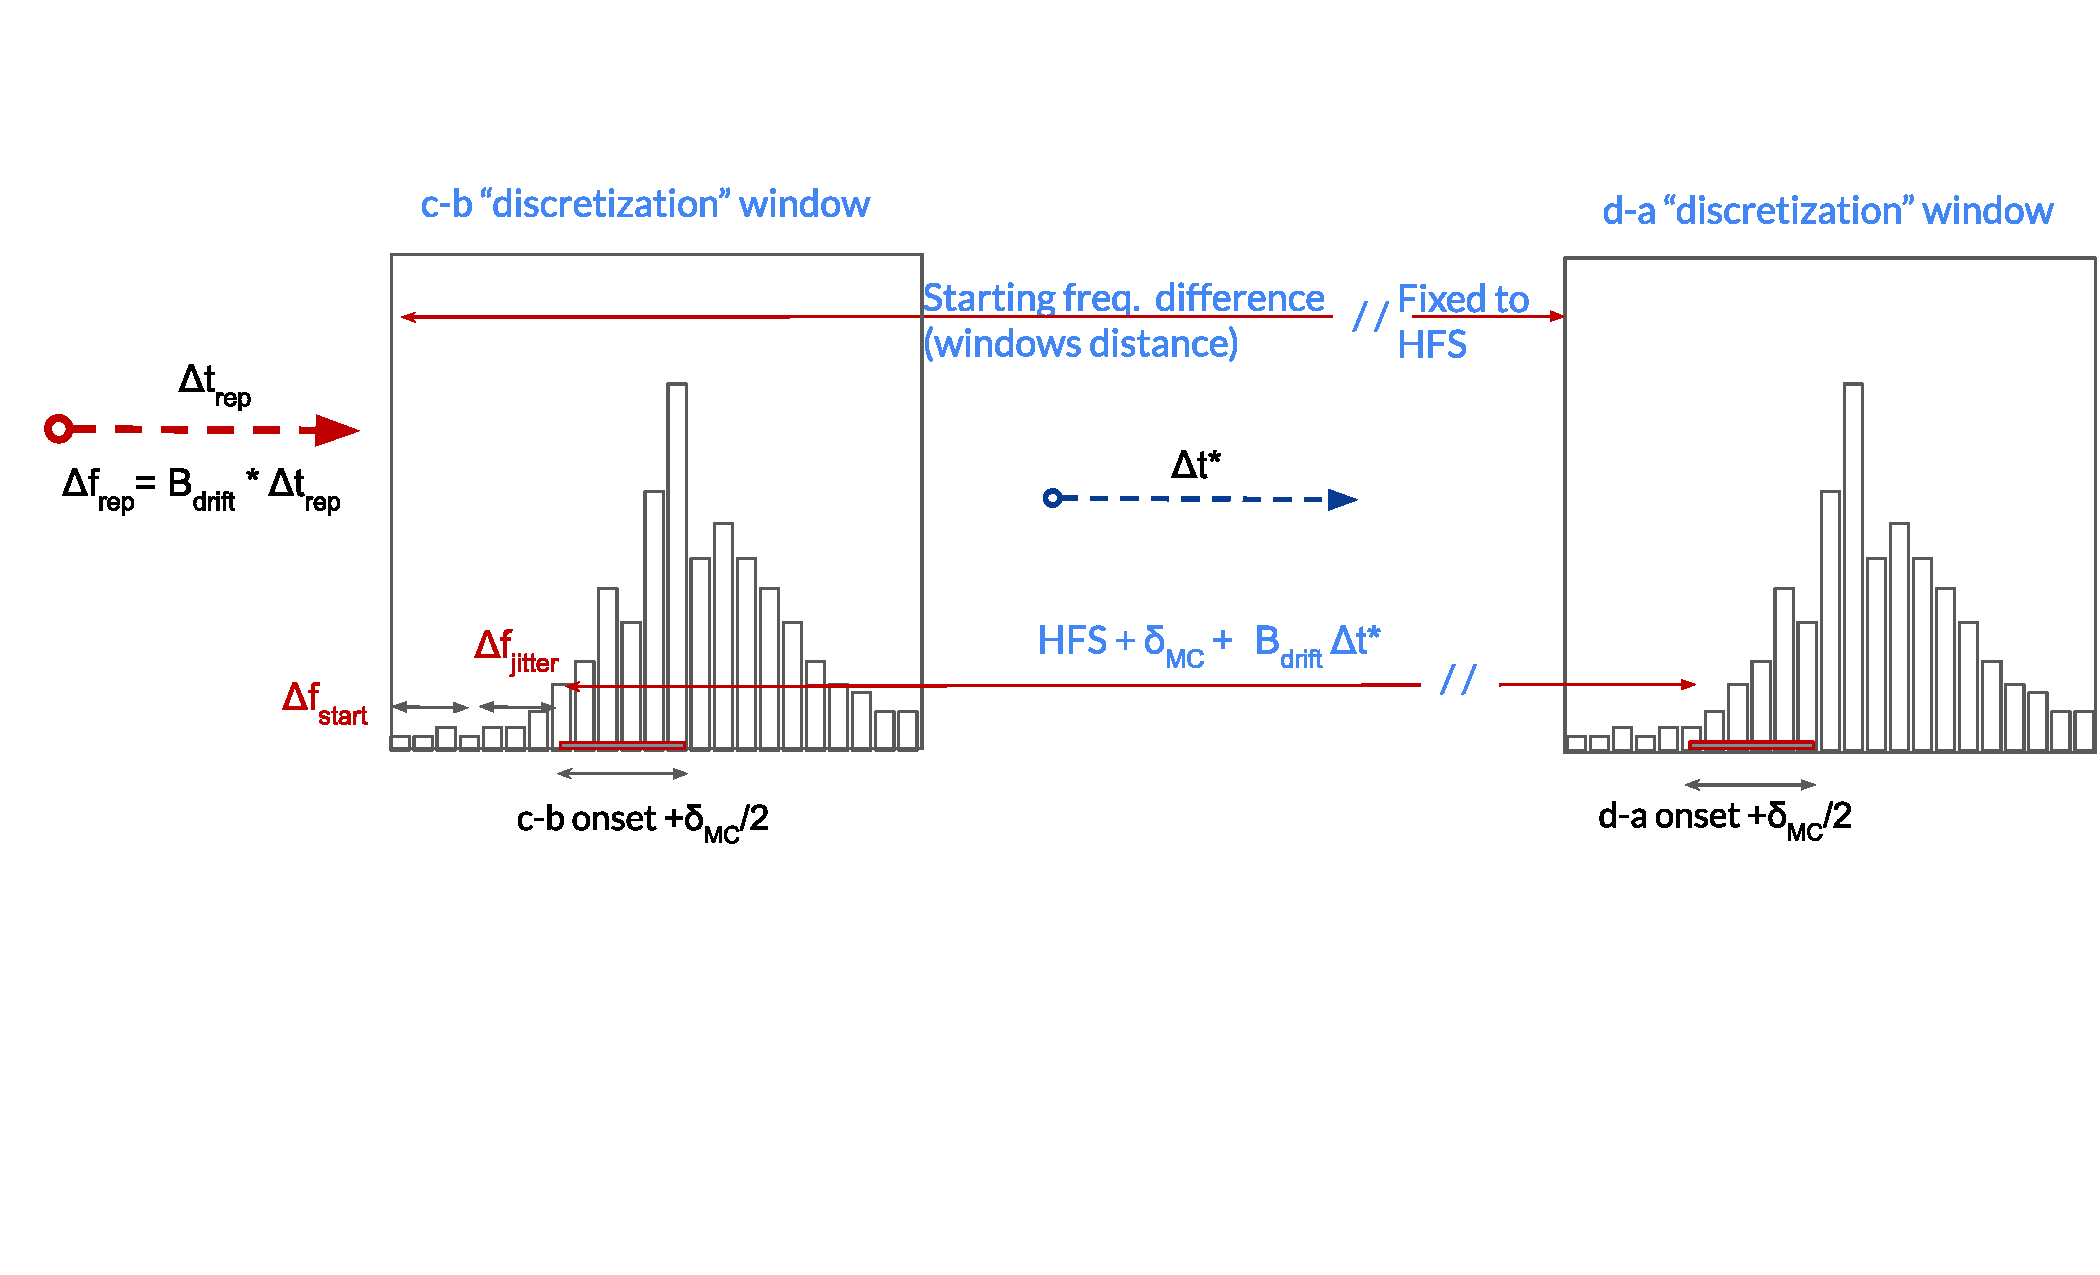
\includegraphics[width = \textwidth]{SchemeRepetition_crop.pdf}
\caption{Scheme of repetition, with all the random implemented to reproduce the experimental uncertainty in the data.}
\label{fig:AschemeRandom}
\end{figure}

\newpage
\subsection{2023 Datasets}

\commento{complete}
During the data taking, 5 different series were acquired, which differs for the the statistic (represented by the number of stack collected before the sampling with the micro-wave light), the frequency step of the sweep, the power of the micro-wave light and the sweep length. A table with all the parameters is reported in \ref{fig:Series} 

\begin{figure}[!h]
\centering
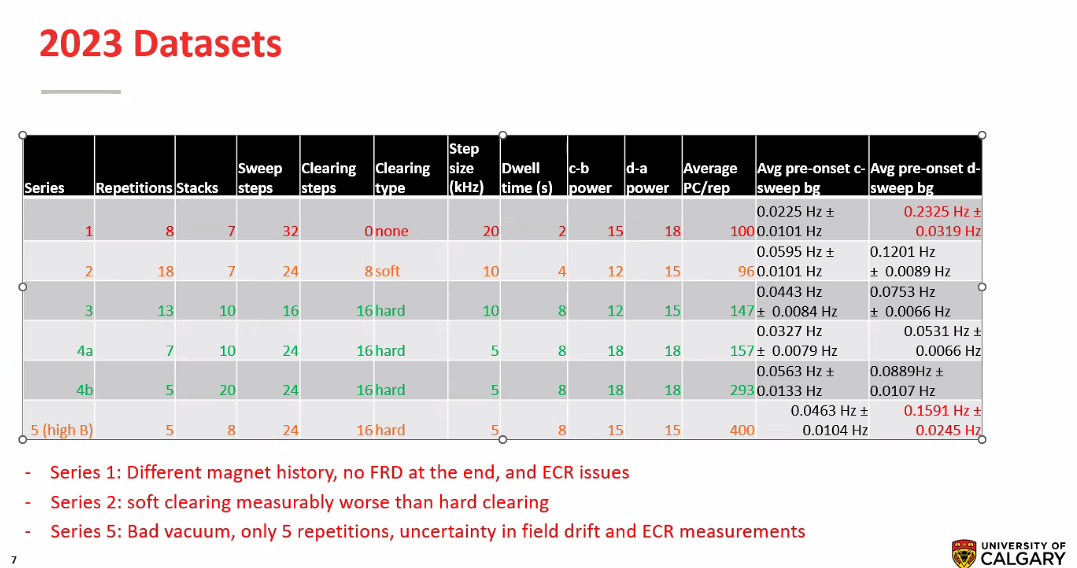
\includegraphics[scale = 0.8, angle = 90]{Screenshot 2024-04-02 183852.png}
\caption{List of series with the experimental parameters}
\label{fig:Series}
\end{figure}

\newpage
\section{PSR Analysis}

\subsection{Onset Finding Algorithms: Definitions}

As mentioned in the introduction, we plan to extract the hyperfine splitting by measuring the onset of individual transitions and then compare the two values with some statistical procedure. In the previous measurement in ALPHA2, the hyperfine splitting has been extracted using an onset finding algorithm, which consist in a scan of over the measured frequencies (starting from the lowest) and selecting the onset as the first frequency where the counts fulfill a certain criteria. The criteria used in 2017 was rather simple, and the onset was selected as the first bin where:

\begin{equation}
onset = i : f_i \geq 1; f_{i + 1} \geq 2 
\end{equation}

Where $f_{i}$ are the counts corresponding to the ith step of the sweep. The Monte Carlo simulation discussed here can be used to study the performance of this algorithm (that from now on will be named the \textbf{forward} algorithm) in the various scenario of the data taking of 2023. 

Some improvements can be made regarding the onset extraction algorithms. Specifically, to mitigate the effect of Poissonian fluctuations in counts, one might consider filtering the lineshape and applying the algorithms to the filtered result. A simple filtering proposal could involve summing N nearby frequencies
Besides this, we have proposed three alternative algorithms, that can be used to improve the results. A first alternative, designed to enhance the robustness of the algorithm in case of different population between d and c states, is the \textbf{constant fraction} algorithm:

\begin{equation}
onset = i : \left(\sum_{i = 0}^{N_{filter}} f_i \right) > cf \cdot N_{filter} \,( TotEntries - N_{filter} \cdot baseline) + N_{filter} \cdot baseline  
\end{equation}

This algorithm adjust the threshold to a fraction of the total events in the transition. The free parameters are the fraction $cf$, and $N_{filter}$ is the parameter which controls the width of the filtering.
A second alternative is based  statistical significance required for a signal to exceed a certain background level. 
This algorithm calculates the threshold based on the observed counts that are a certain number of standard deviations above the background. The mathematical definition of this significance algorithm (from now on named \textbf{significance}) is given in equation \ref{eq:Significance}

\begin{equation} \label{eq:Significance}
onset = i : \left( \sum_{i = 0}^{N_{filter}} f_i \right) > N_{filter} \, N_{\sigma}^{2} + 2 N_{\sigma} \sqrt{N_{filter} \cdot baseline} 
\end{equation}

The last algorithm that we have considered is the \textbf{reversed} algorithm, which is similar to the forward one except that the scan starts from the highest frequencies and moves towards the lowest, and the threshold criteria are "specular"

\begin{equation}
onset = i : f_i \leq 1; f_{i - 1} \leq 2 
\end{equation}

\subsection{Hyperfine Splitting Extraction: Combined Fit}

We have highlighted in equation \ref{eq:hfsmes} that the hyperfine splitting can be extracted knowing the value of the magnetic field drift. Once we have extracted the onset from each of repetitions of a dataset, the analysis consist on performing a combined linear fit to the data with the model:

\begin{align}
onset_{da}(t) = slope \cdot t + q_{2} \\
onset_{cb}(t) = slope \cdot t + q_{1}
\end{align} 

Where the da and cb onsets are fitted separately with a linear model, with the constraint that the slope is common in both models. The hyperfine splitting will be given by the formula:

\begin{equation}
hfs = q_{2} - q_{1}
\end{equation}

\begin{figure}[hbtp]
\centering
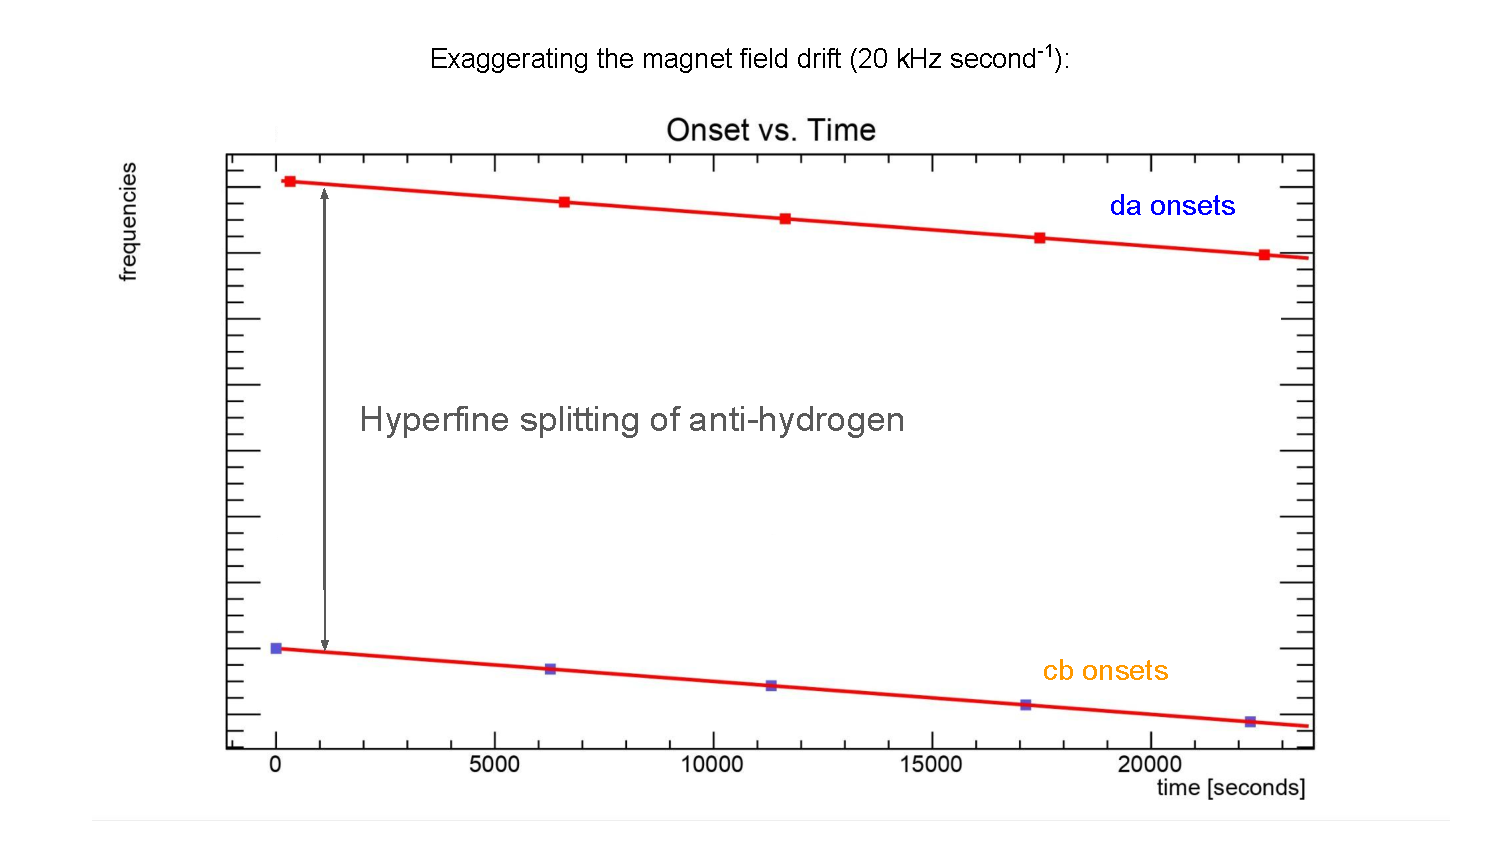
\includegraphics[width = \textwidth]{Fit.pdf}
\caption{ Example of combined fit. The slope is common for the two series of data, while there are two intercepts free to vary.}
\end{figure}

The simulation produces in output a certain number of datasets, where each dataset is a single realization of the experiment, namely a "trial". The fit procedure is repeated on each trial, and the list of result are valuable to compute important quantities as the statistical uncertainty and bias. More explicitly:

\begin{equation}
\sigma_{hfs}^2 = E[(hfs_{measured} - hfs_{MC})^2]
\end{equation} 

where $E[(hfs_{measured} - hfs_{MC})]$ is the expectation value of the residual between the outcome of the analysis, $hfs_{measured}$, and the value that was used as the input of the Monte Carlo, $hfs_{MC}$. For the slope we have similarly

\begin{equation}
\sigma_{slope}^2 = E[(slope_{measured} - B_{drift \; MC})^2]
\end{equation}

it is also interesting to study the mean of the residual, which represents the bias of the experimental protocol:

\begin{equation}
bias_{hsf} = E[(hfs_{measured} - hfs_{MC})]
\end{equation}

and similary for the slope.

\section{Transitions Asymmetries and Systematic errors}
\commento{ Discuss all the possible source of asymmetries which can influence the measurement}


\newpage
\subsection{Parameter Optimization}
\commento{ explain how the optimization works, which is the optimization space and the various types of optimization, which are:
\begin{itemize}
\item optimization without asymmetries.
\item optimization with asymmetric background due to residual gas.
\item optimization with asymmetric rise time.
\item optimization with asymmetric statistic.
\end{itemize}
}

\begin{figure}[!hbtp]
\centering
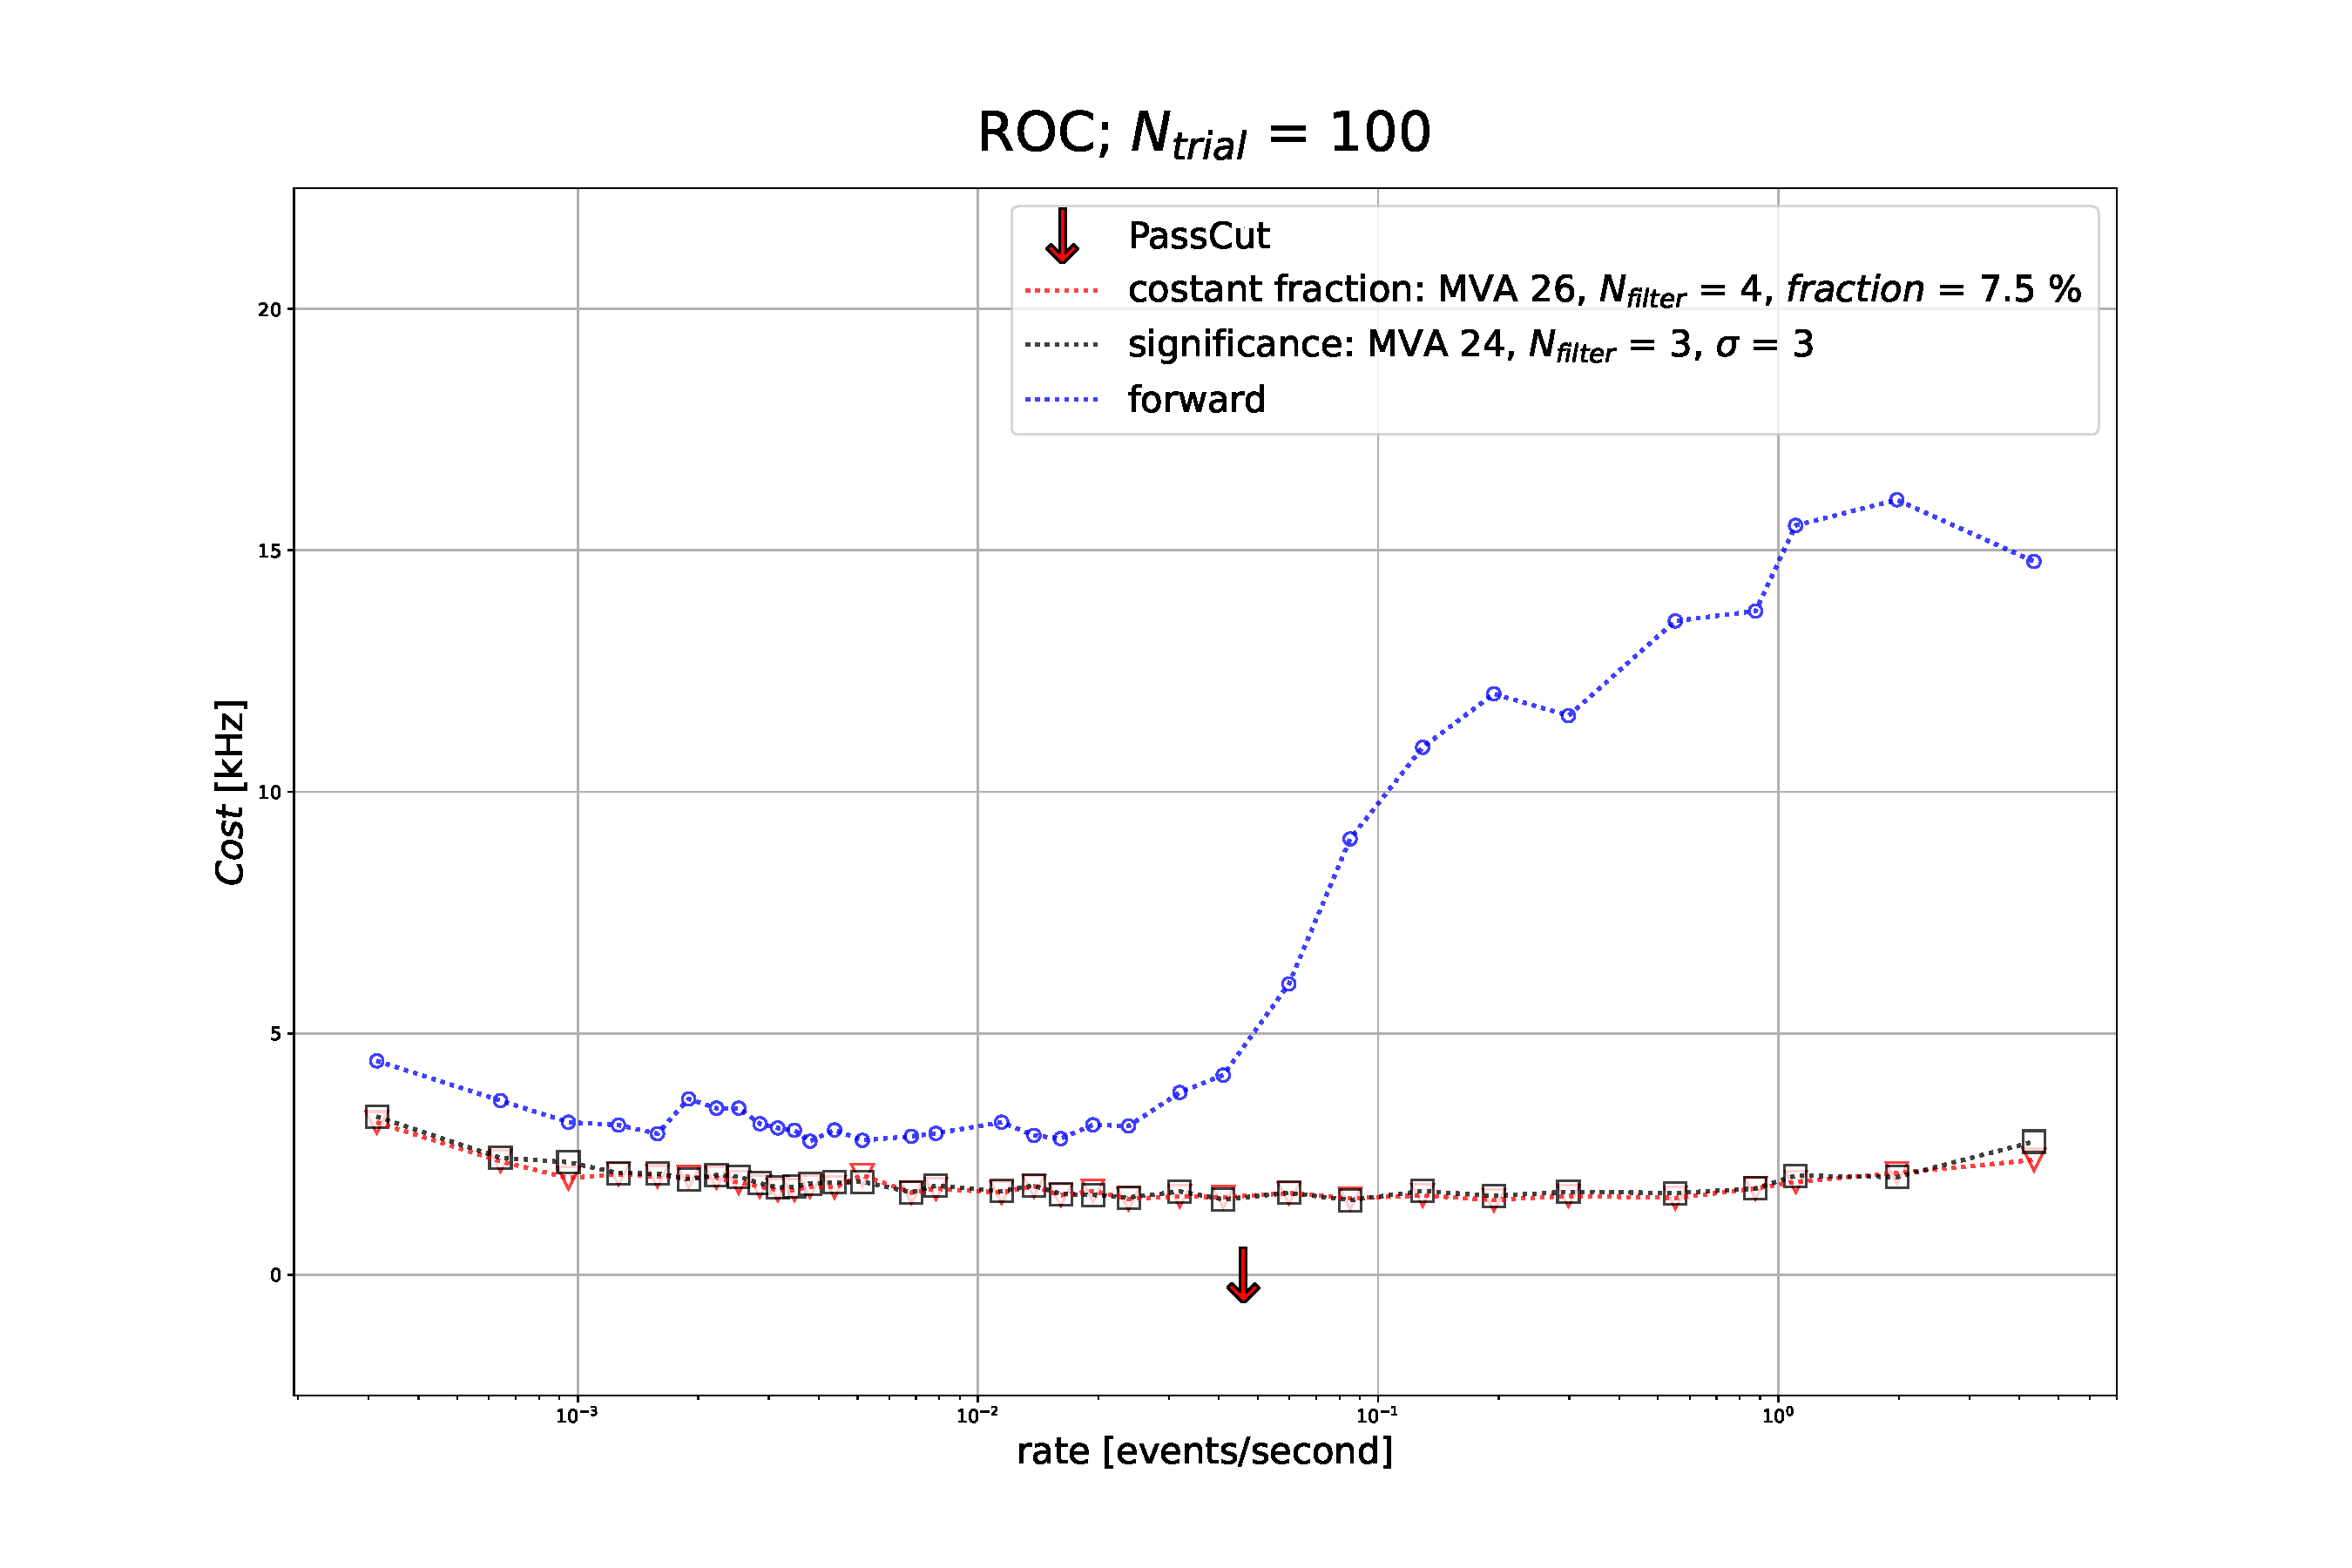
\includegraphics[width = 0.9\textwidth]{ROC_variance_bias.pdf}
\caption{Optimization of three different onset-finding algorithms for the 4b scenario.}
\commento{qui non ho fatto l'ottimizzazione scalando per il fondo!}
\end{figure}

\newpage
\subsection{Systematic Effects due to Magnetic field drift}

The magnetic field $\vec{B}$ in the anti-hydrogen trap can produce several effects that influence the hyperfine splitting measurement. For instance, magnetic field in-homogeneity could locally modify the frequency transition for a part of the trapped $\overline{H}$, broadening the spectroscopic line of the transition. Also
the variation of the magnetic field due to time influence both onset frequency and \textit{cb}/\textit{da} transition shape. The magnetic field drift $\vec{B}_{drift}$ (measured in $\SI{}{\kilo \hertz \second\tothe{-1}}$) is supposed to be constant over time, with magnitude of $ \simeq \SI{0.02}{\kilo \hertz \second\tothe{-1}}$ or equivalently $ \simeq \SI{70}{\kilo \hertz \hour\tothe{-1}}$.

The shape of the transition  is modified due to the fact that the experimental measurement at each frequency are made a different times. Denoting the transition as $\psi(t,f,\vec{B})$ where we have made the time, frequency and $\vec{B}$ dependence explicit, the measurement are at each frequency are given by:

\begin{eqnarray*}
f_{0}& : &\psi(f_{0},B(t))   \\
f_{1}& : &\psi(f_{1},B(t + \delta_{tstep})) = \psi(f_{0},B(t) - B_{drift} \cdot \delta t) \\
f_{2}& : &\psi(f_{2},B(t + 2\delta_{tstep})) = \psi(f_{0},B(t) - B_{drift} \cdot 2 \delta t)\\
... & ...
\end{eqnarray*}

In principle this effects could be simulated with a discretization of the line-shape which accounts for the explicit dependence over time. Despite this, for low magnitude of $B_{drift}$, the shift produced is of the order of $\SI{0.02}{\kilo \hertz \second \tothe{-1}} \cdot \delta t_{step} = \SI{0.16}{\kilo \hertz}$, having imposed $\delta t_{step} =\SI{8}{\second}$. The effect is relatively small compared to the frequency increment of $\SI{5}{\kilo \hertz}$ for each step. Despite this, since this effect accumulates over time, the biggest effect will occur for higher frequencies at the end of the sweep. For the very last been of the sweep, we expect to have $ \SI{0.16}{\kilo \hertz} \cdot 24  = \SI{3.84}{\kilo \hertz} $, where 24 is number of step in a single. In this case the result is comparable with the frequency sampling of 5 kHz, nevertheless this only modifies the shape of the right tail of the lineshape, with a negligible influence on the onset determination.

A more significant effects, which is considered in the simulation, is directly related to the change over time of the onsets frequencies. Since the onsets of the \textit{cb} and \textit{da} transition are measured at a different time, the hyperfine splitting of anti-hydrongen, measured as the difference between the two onsets, is directly influenced by the $B_{drift}$ effect. 

\begin{figure}[!hbtp]
\centering
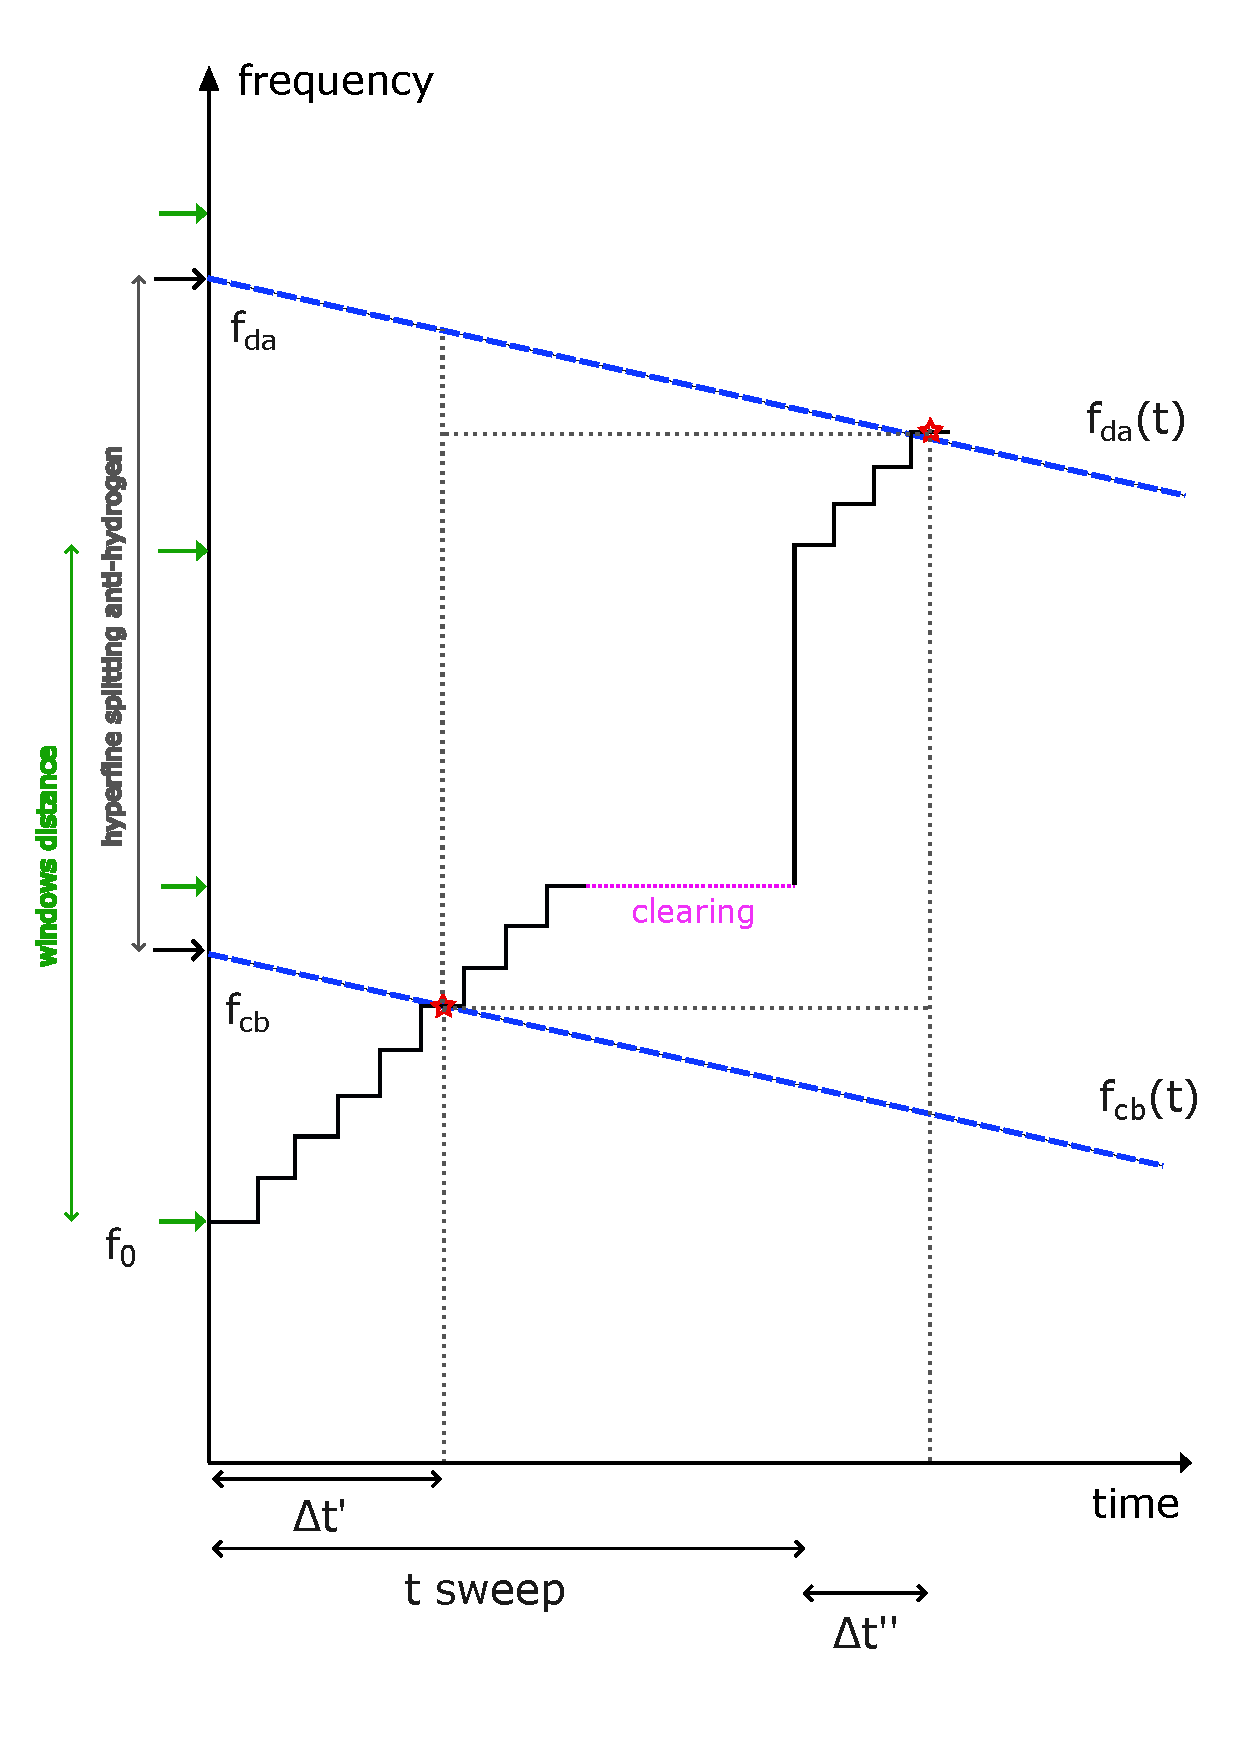
\includegraphics[scale= 0.8]{SchemeBdrift.pdf}
\caption{Scheme of Bdrift effects on onset determination}\label{fig:SchemeBdrift}
\end{figure}


A quantitative estimation of this effect is calculated from the scheme shown in figure \ref{fig:SchemeBdrift}. The onset \textit{cb} is found when the blue line (which represent the variation of the onset frequency given by the $B_{drift}$ effects) intersects the step by step rising frequency of the micro wave laser used to induce the transitions. Considering an ideal algorithm without uncertainty, this is equivalent to:

\begin{equation} \label{eq:cbOnset}
f_{0} + \dfrac{f_{step}}{t_{dwell}} \cdot \Delta t' = f_{cb}(t) = f_{cb} - B_{drift} \cdot \Delta t'
\end{equation}

Resolving this equation in the variable $\Delta t'$, the time at which the onset is found, gives:

\begin{equation}
\Delta t' = \dfrac{f_{cb} - f_{0}}{ \frac{f_{step}}{t_{dwell}} + B_{drift}}
\end{equation}

Substituting in $f_{cb}(t)$ gives the measured onset for the \textit{cb} transition:

\begin{equation}
f_{cb}(t = \Delta t') = f_{cb} - B_{drift} \dfrac{f_{cb} - f_{0}}{ \frac{f_{step}}{t_{dwell}} + B_{drift}}
\end{equation} 

The onset for \textit{da} transition can be found with the same method, although we have to consider an additional time interval made up by the last frequency steps of the \textit{cb} transition and the 16 clearing step. With this additional information we can derive the equivalent equation of the \ref{eq:cbOnset}

\begin{equation}
f_{0} + hfs +  \dfrac{f_{step}}{t_{dwell}} \cdot \Delta t'' = f_{da} -B_{drift} \cdot (t_{sweep} + \Delta t'') 
\end{equation}

where $hfs$ indicates the frequency distance between the two starting point of the sweep (equal to the hyperfine splitting of hydrogen). The time $\Delta t''$ is:

\begin{equation}
\Delta t'' = \dfrac{f_{da} - B_{drift} \cdot t_{sweep} - f_{0} - hfs}{ \frac{f_{step}}{t_{dwell}} + B_{drift}}
\end{equation} 

As before, substituting in $f_{da}$ gives the result:

\begin{equation}
f_{da} - B_{drift} t_{sweep} - B_{drift} \dfrac{( f_{da} - B_{drift} t_{sweep} - f_{0} - hfs)}{ \frac{f_{step}}{t_{dwell}} + B_{drift}}
\end{equation}

It is interesting now to study the difference between the two onset, which allows to identify quantitatively how much the $B_{drift}$ influence the measurement. 

\begin{equation} \label{eq:Systematiceffect}
\overline{hfs}_{measured} = \overline{hfs} - B_{drift} \cdot t_{sweep} - B_{drift}  \dfrac{(\overline{hfs} - hfs - B_{drift} \cdot t_{sweep})}{ \frac{f_{step}}{t_{dwell}} + B_{drift}}
\end{equation}

If the $B_{drift}$ are small compared to $\frac{f_{step}}{t_{dwell}}$, we can simplify the expression above, obtaining:

\begin{equation}
\overline{hfs}_{measured} = \overline{hfs} - B_{drift} \cdot \biggl(t_{sweep} + \frac{ \overline{hfs} - hfs}{\frac{f_{step}}{t_{dwell}}} \biggl) + \, B_{drift}^{2} \cdot \biggl( t_{sweep} \, \frac{t_{dwell}}{f_{step}} \biggl)
\end{equation}

two additional terms are present, one which is proportional to the magnetic field drift, and one proportional to the square.

\begin{figure}[!hbtp]
\centering
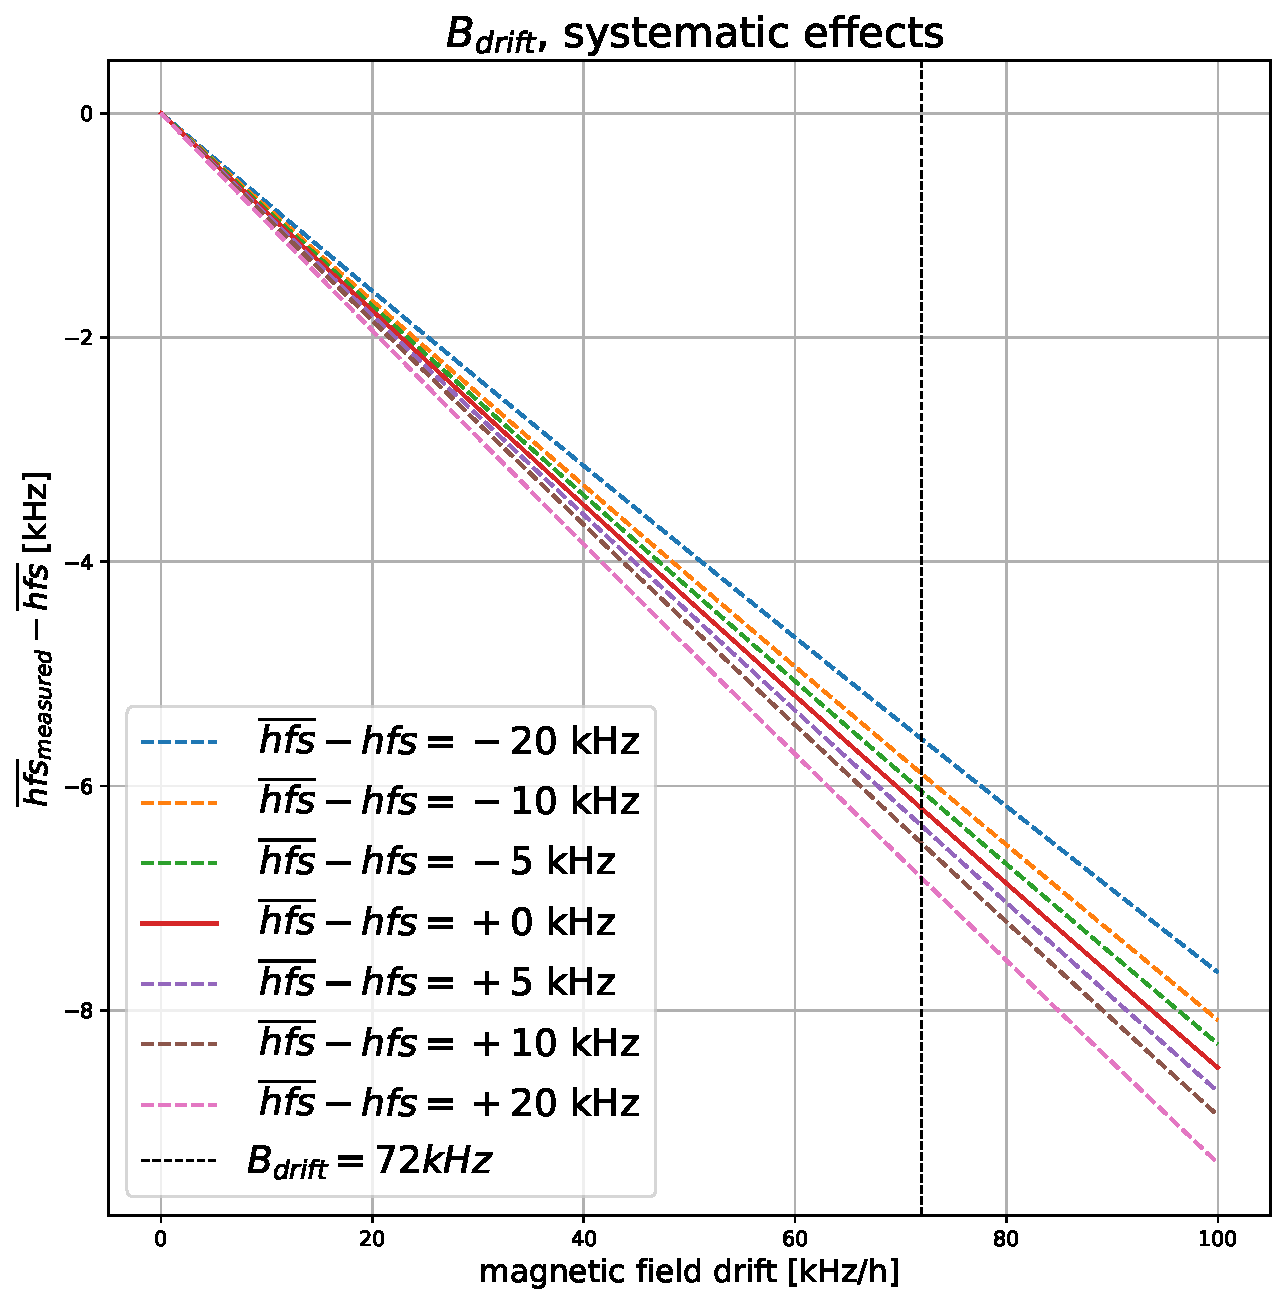
\includegraphics[width = 0.75\textwidth]{driftFirstOrder.pdf}
\caption{Plot of the systematic error due to $B_{drift}$, as computed in \ref{eq:Systematiceffect}. The plot represents 5 different possible scenarios which differentiate for the hyperfine-splitting of anti-hydrogen with respect to hydrogen ($\overline{hfs} - hfs$) }
\label{fig:SystematicB}
\end{figure}

\newpage
The first correction term, $- B_{drift} \cdot t_{sweep}$ is corrected by the fit linear fit procedure. Nevertheless, a second order term is also present, whose presence affects the measurements as shown in figure \ref{fig:SystematicB}

\begin{figure}[!hbtp]
\centering
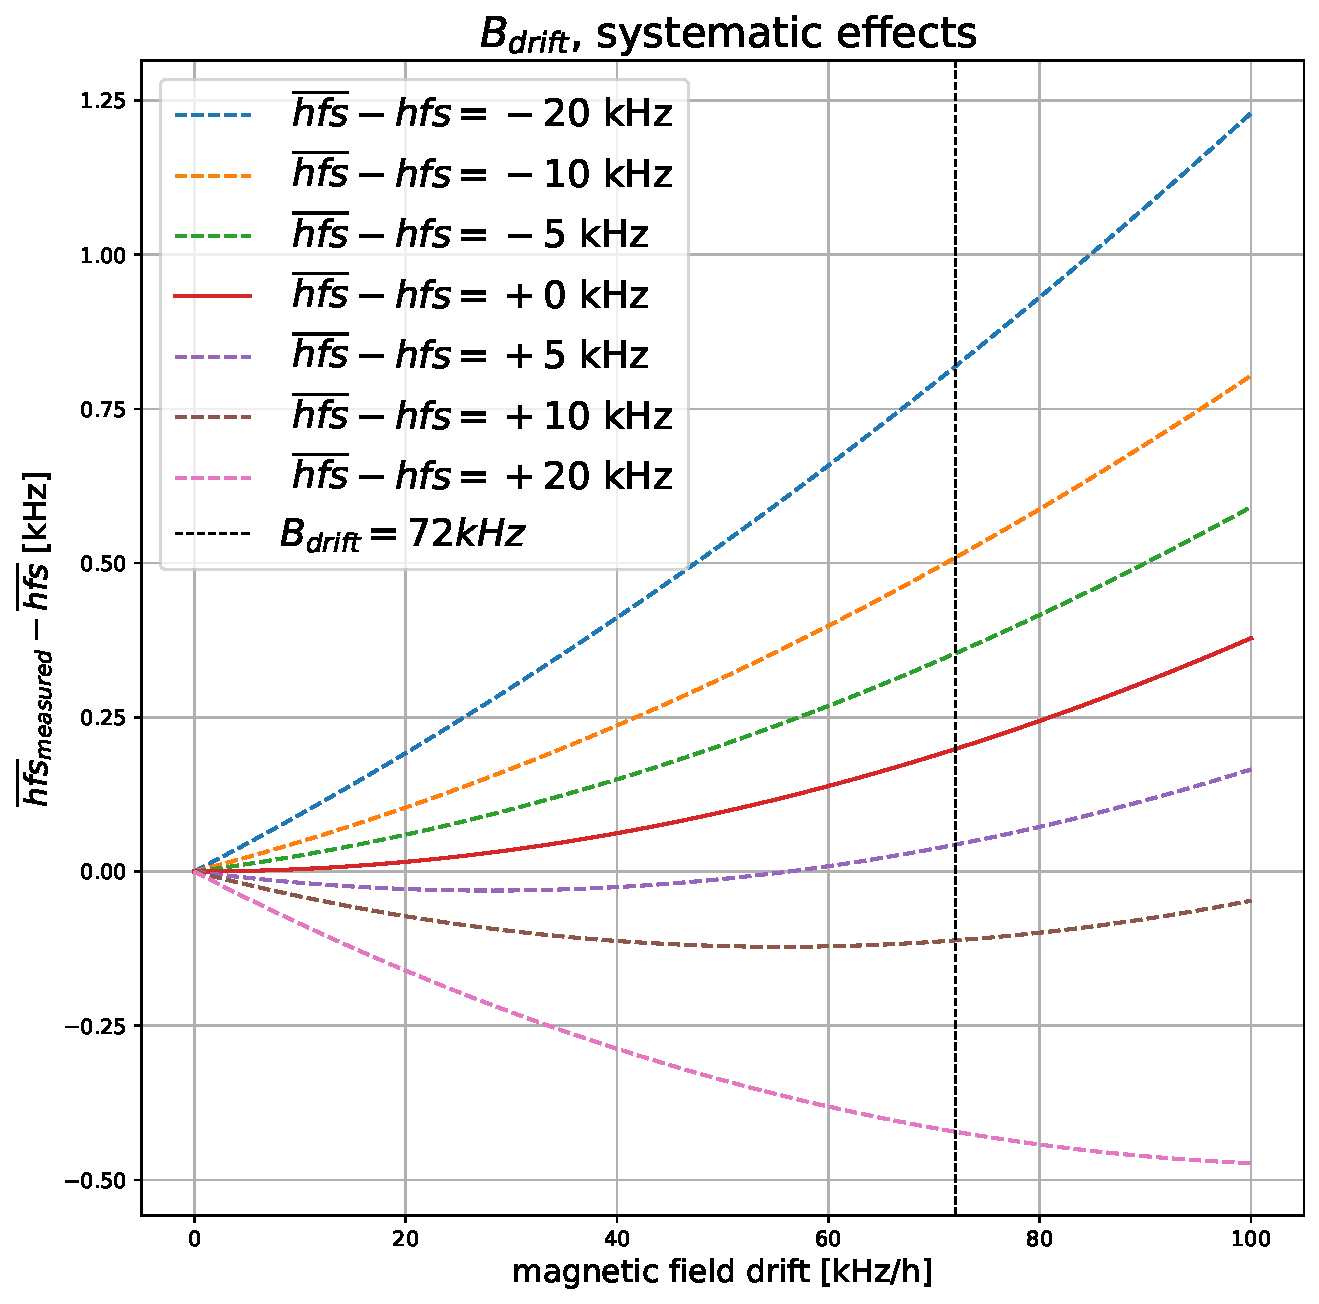
\includegraphics[width = 0.75\textwidth]{driftSecondOrder.pdf}
\caption{Plot of the second order term of equation \ref{eq:Systematiceffect}. The $B_{drift}$ effects are computed for 5 different possible scenarios with a different hyperfine splitting of anti-hydrogen with respect to hydrogen ($\overline{hfs} - hfs$) }
\label{fig:driftSecondOrder}
\end{figure}

\newpage
\section{Results}

\subsection{Summary Tables}
\begin{table}[hbtp]
\centering
\begin{tabular}{||p{20mm}|c|c|c||}
\textcolor{red}{Background} \newline \textcolor{red}{asymmetry} & forward & constant fraction & significance \\ 
\hline 
series 3 & • & • & • \\ 

series 4a & • & • & • \\ 
 
series 4b & $\mu = -2.189 \quad \sigma = 5.02$ & $\mu = -0.46 \quad \sigma = 2.49$ & $\mu = 0.004 \quad \sigma = 2.51$ \\ 
 
\end{tabular}
\caption{Every value is expressed in $kHz$, the simulation is tuned to the \textbf{PASSCUT} efficiency and cosmic rate values}
\end{table}

\begin{table}[hbtp]
\centering
\begin{tabular}{||p{40mm}|ccc||}
\textcolor{blue}{rise asymmetry \newline [40 kHz cb, 50 kHz da]} & forward & constant fraction & significance \\ 
\hline 
series 3  & • & • & • \\ 

series 4a & • & • & • \\ 
 
series 4b & $\mu = +4.8 \quad \sigma = 3.8$  & $\mu = +6 \quad \sigma = 2.52$ & $\mu = +8.23 \quad \sigma = 2.9$ \\ 
 
\end{tabular} 
\caption{Every value is expresse in $kHz$, the values are tuned to the \textbf{PASSCUT} efficiency and cosmic rate values}
\end{table}

\begin{figure}[hbtp]
\centering
\textbf{SYSTEMATIC AND STATISTICAL UNCERTAINTY (FORWARD ALGORITHM)} \\ \vspace{10pt}
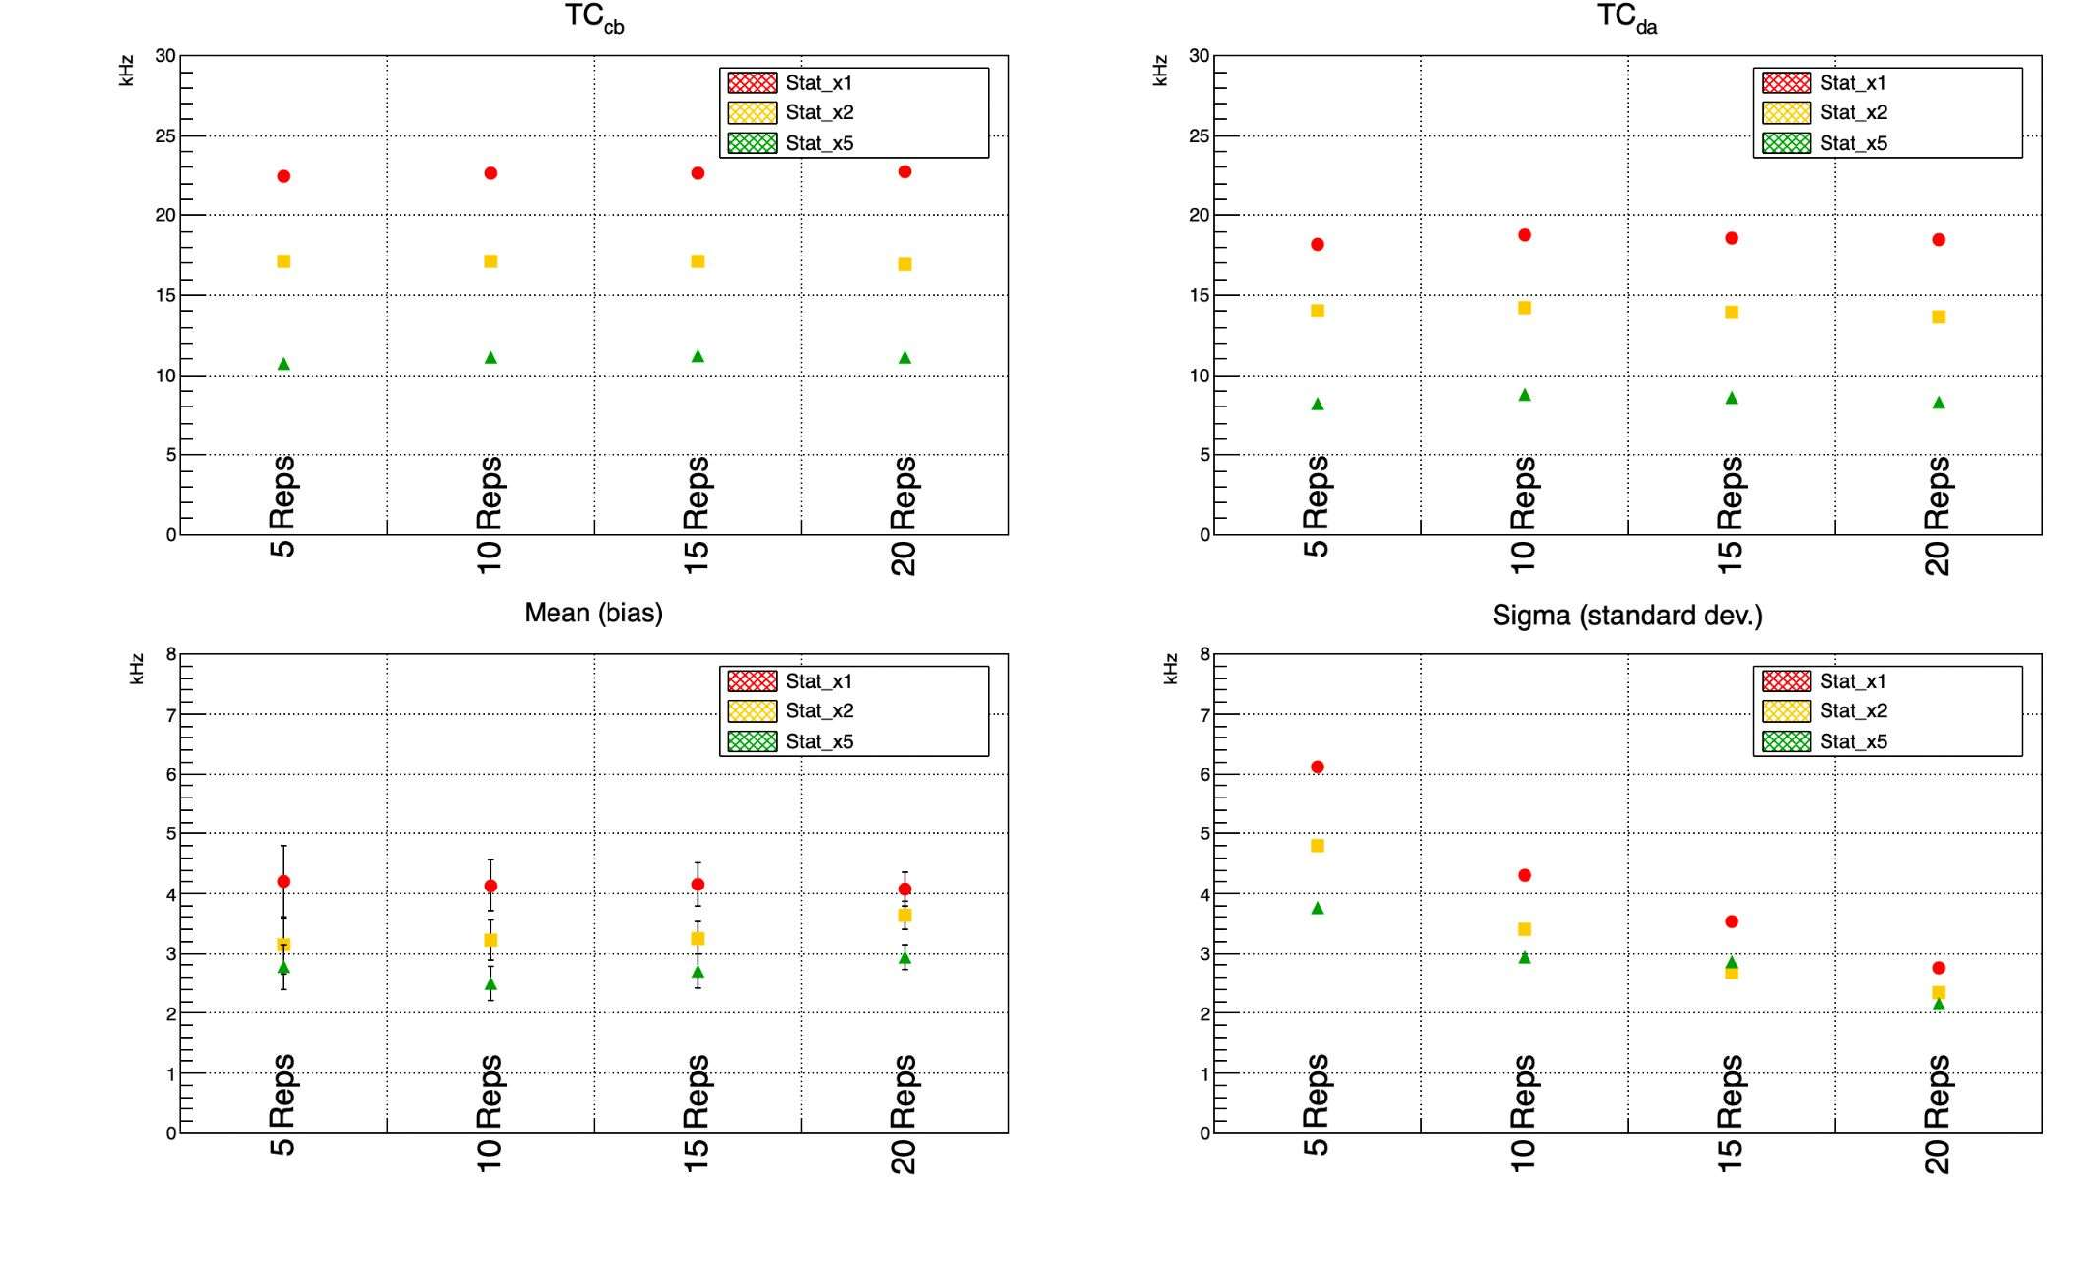
\includegraphics[width = 0.8\textwidth]{statistic-variation.pdf}
\caption{Behavior as a function of the number of repetitions of the statistical error and the bias of the measurement of the hyperfine splitting, for a varying number of accumulated antihydrogens}
\commento{Rifare con il fondo che scala in base alla statistica utilizzata}
\end{figure}

\newpage
\subsection{4b scenario}

The tested algorithms are the forward, the constant fraction and the significance. The parameters are:

\begin{itemize}
\item constant fraction : $N_{filter} = 4 \quad ; \quad fraction = 7.5\%$ 
\item significance : $N_{filter} = 3 \quad ; \quad N_{\sigma} = 3$
\item forward : $\geq 1 \quad ; \quad \geq 2 $
\end{itemize}

\subsubsection{Asymmetric Background}
\begin{figure}[hbtp]
\centering
\textbf{FORWARD ALGORITHM 4B SERIE} \vspace{10pt}\\
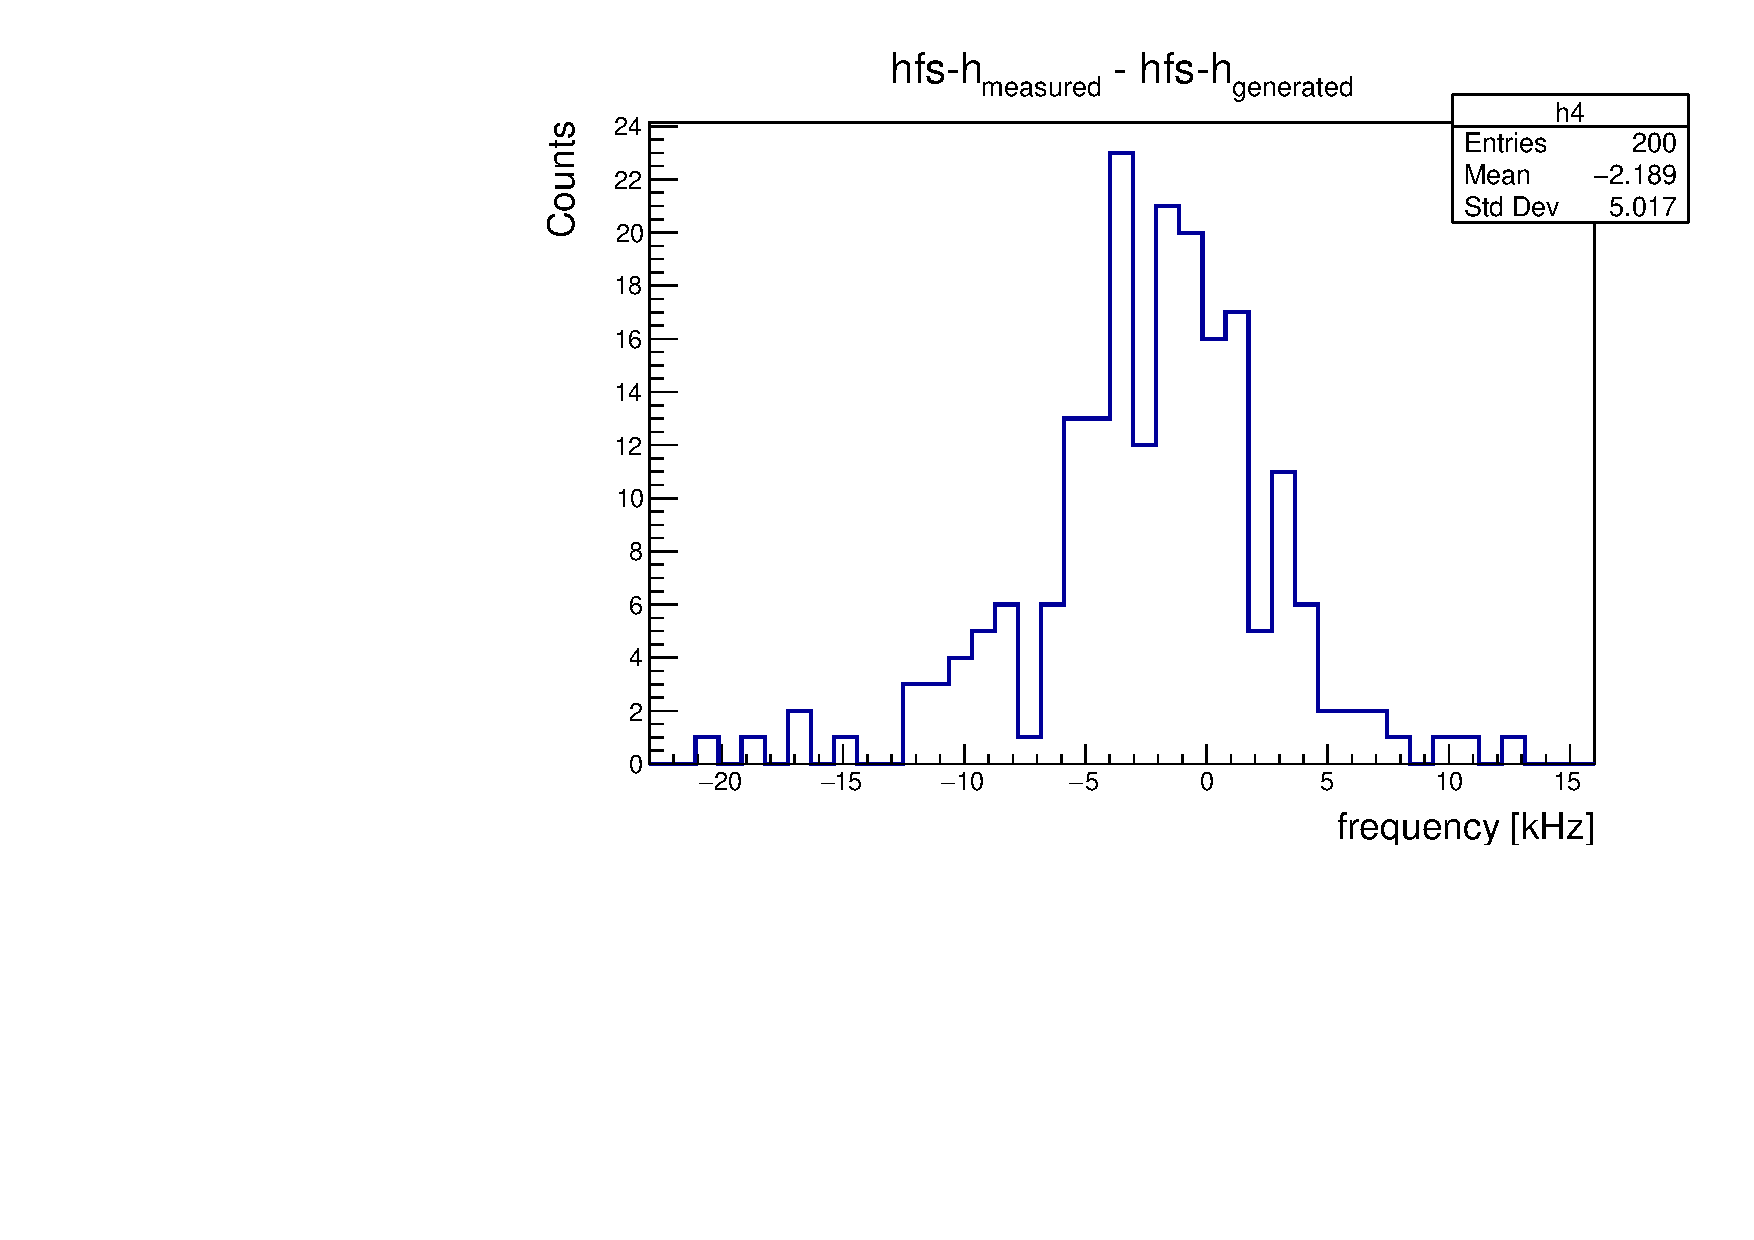
\includegraphics[width = 0.49\textwidth]{forward/4bmuonONresgasON.pdf}
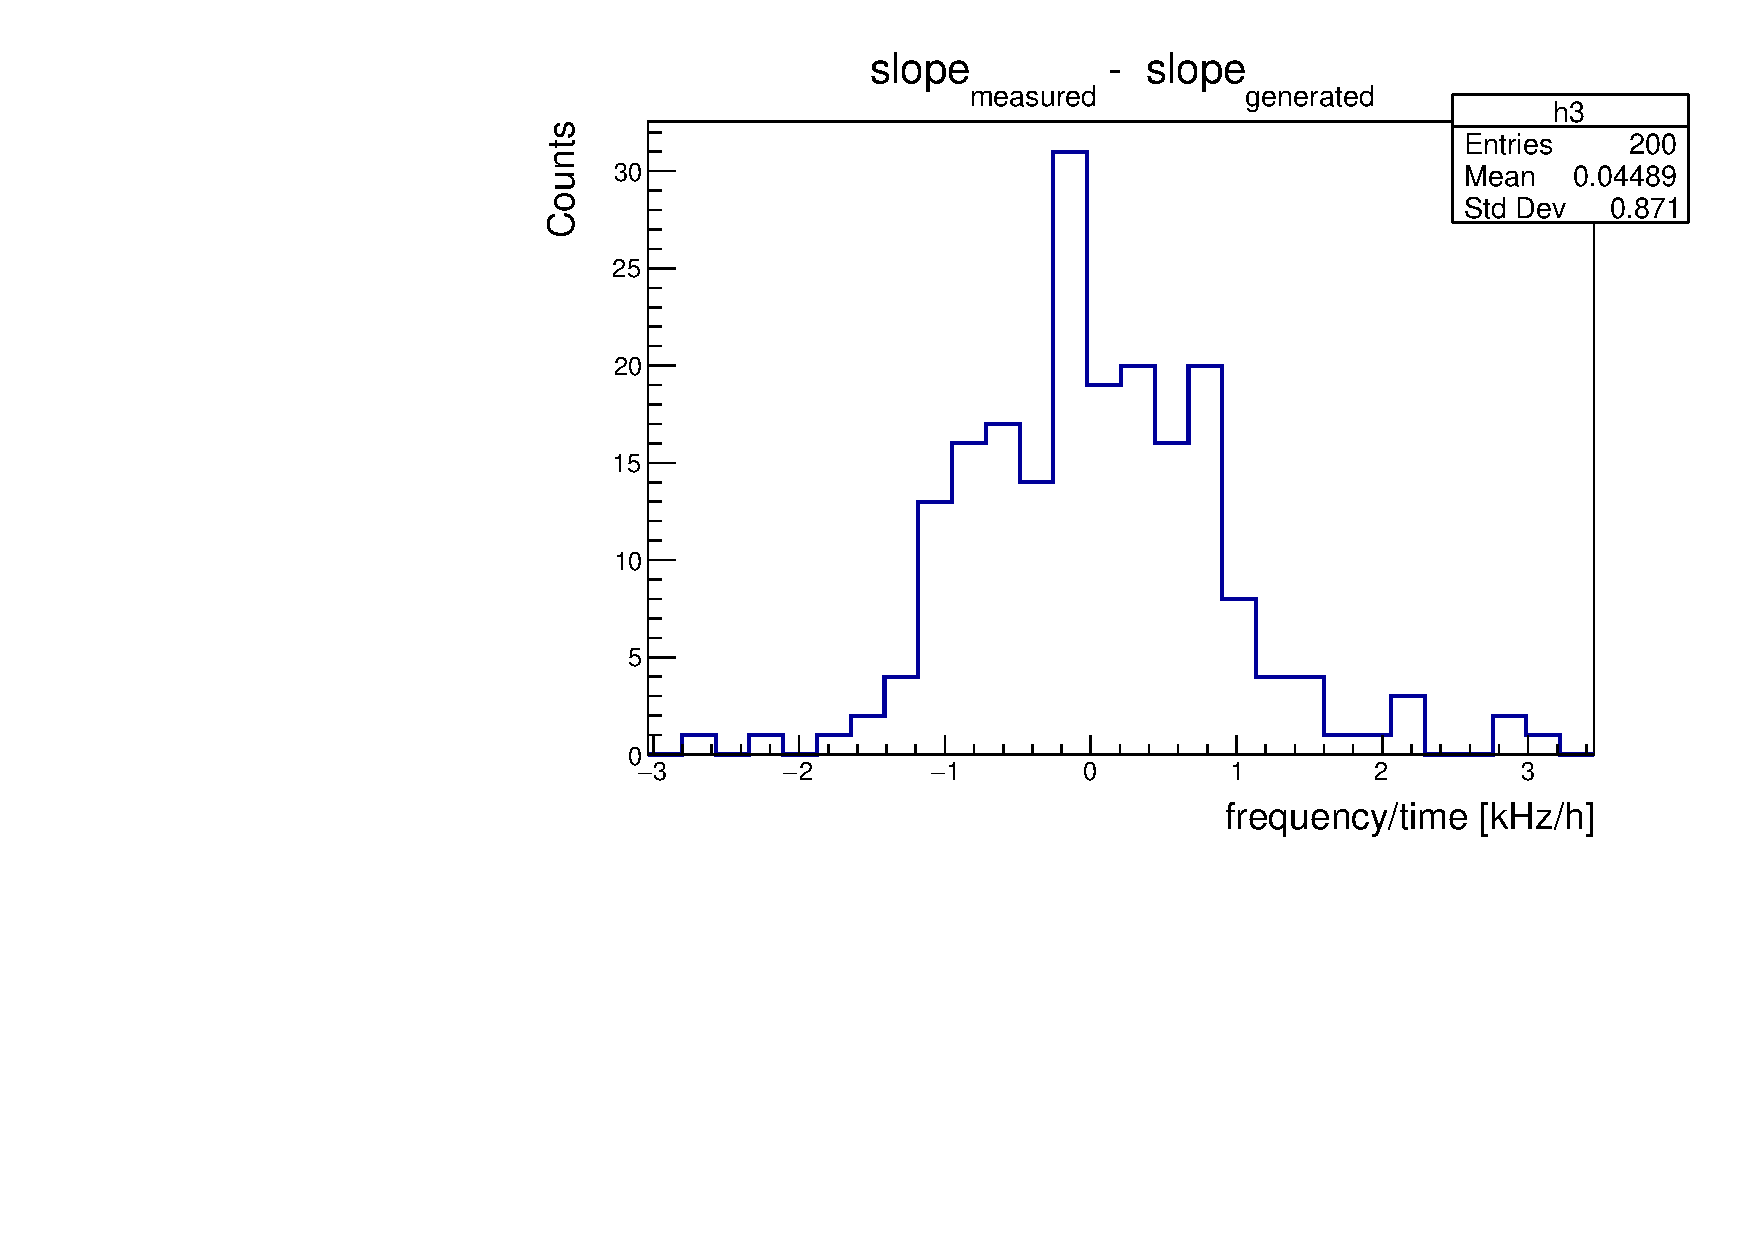
\includegraphics[width = 0.49\textwidth]{forward/4bmuonONresgasON_slope.pdf}
\caption{4b scenario, on the left the residual between the measured and the Monte Carlo true value hyperfine splitting, on the right the residual between the estimated and the true value of the magnetic drift.}
\end{figure}

\begin{figure}[hbtp]
\centering
\textbf{CONSTANT FRACTION ALGORITHM 4B SERIE} \vspace{10pt}\\
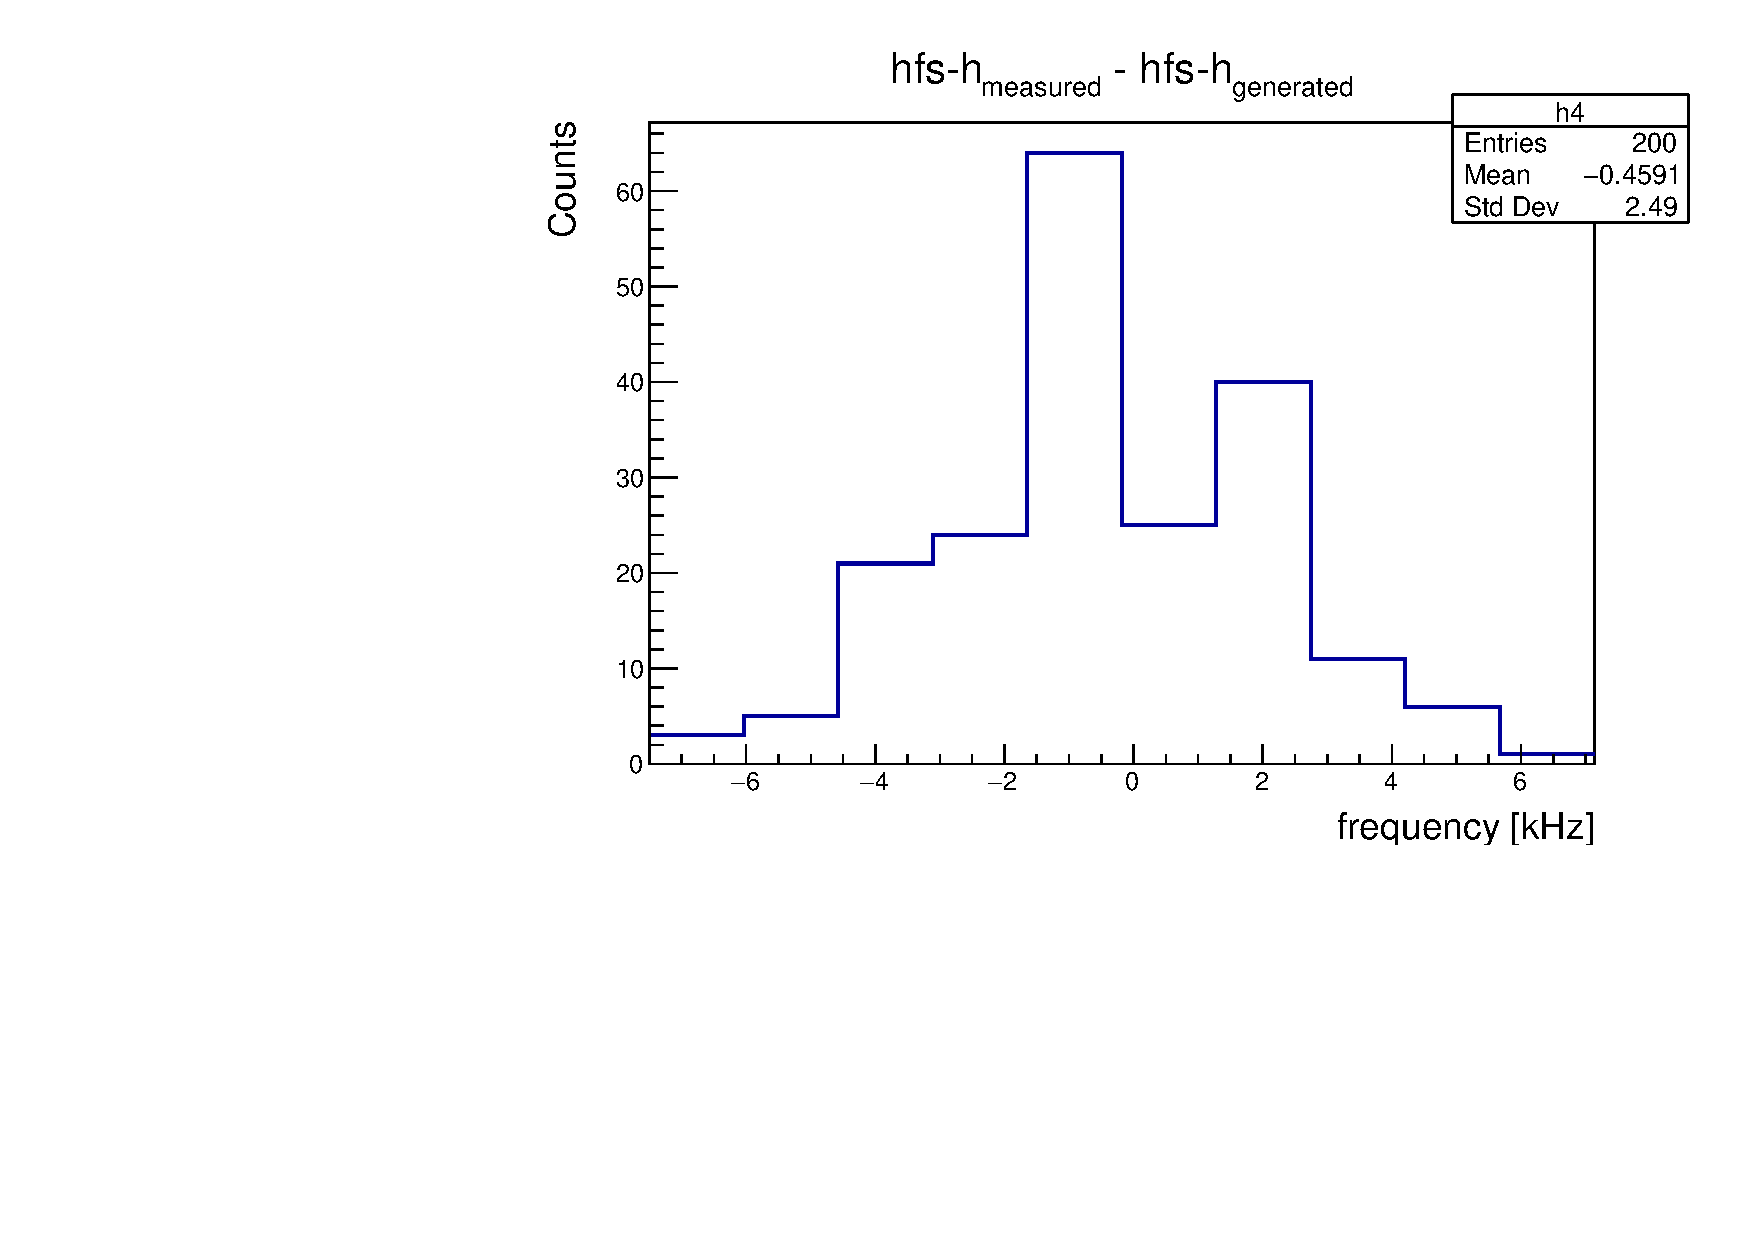
\includegraphics[width = 0.49\textwidth]{constantfraction/4bmuonONresgasOn.pdf}
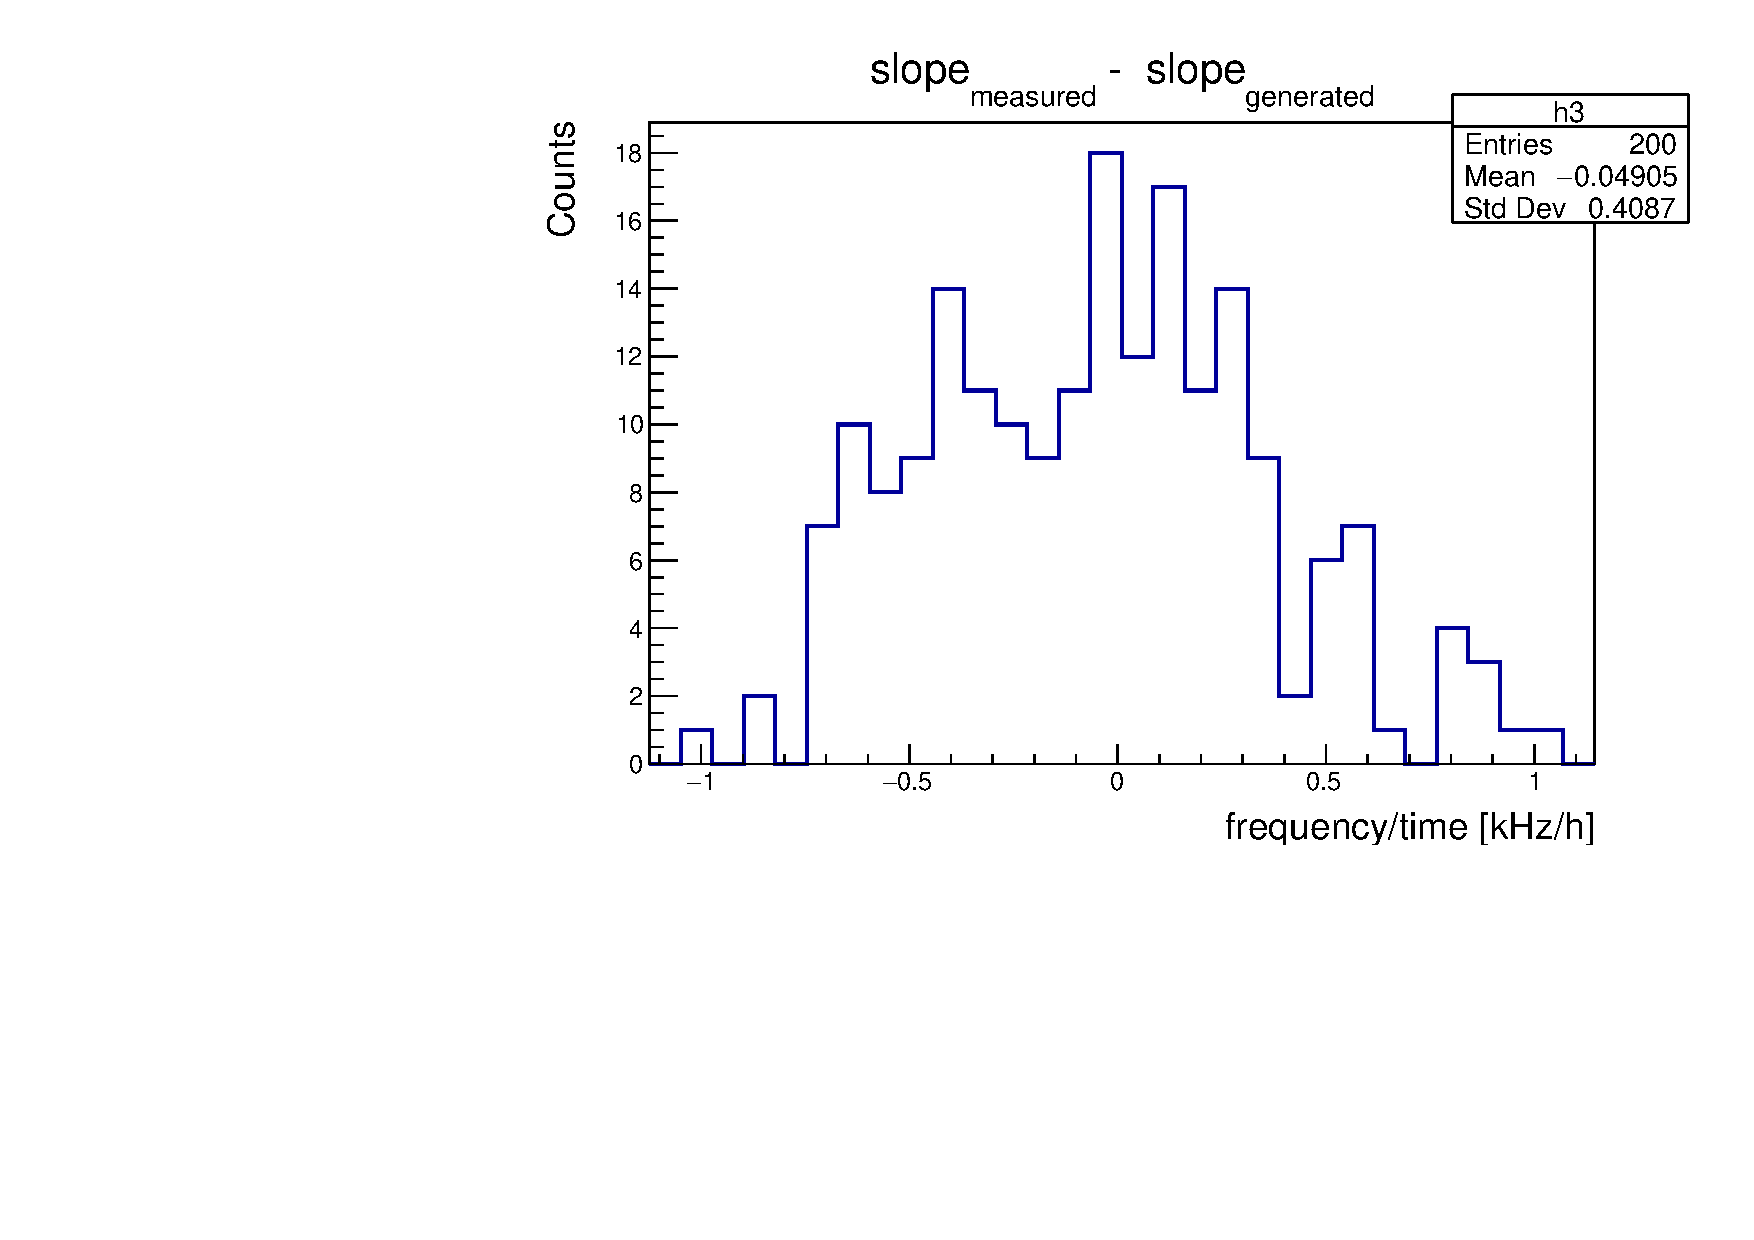
\includegraphics[width = 0.49\textwidth]{constantfraction/4bmuonONresgasOn_slope.pdf}
\caption{4b scenario, on the left the residual between the measured and the Monte Carlo true value hyperfine splitting, on the right the residual between the estimated and the true value of the magnetic drift.}
\end{figure}

\begin{figure}[!hbtp]
\centering
\textbf{SiGNIFICANCE ALGORITHM 4B SERIE} \vspace{10pt}\\
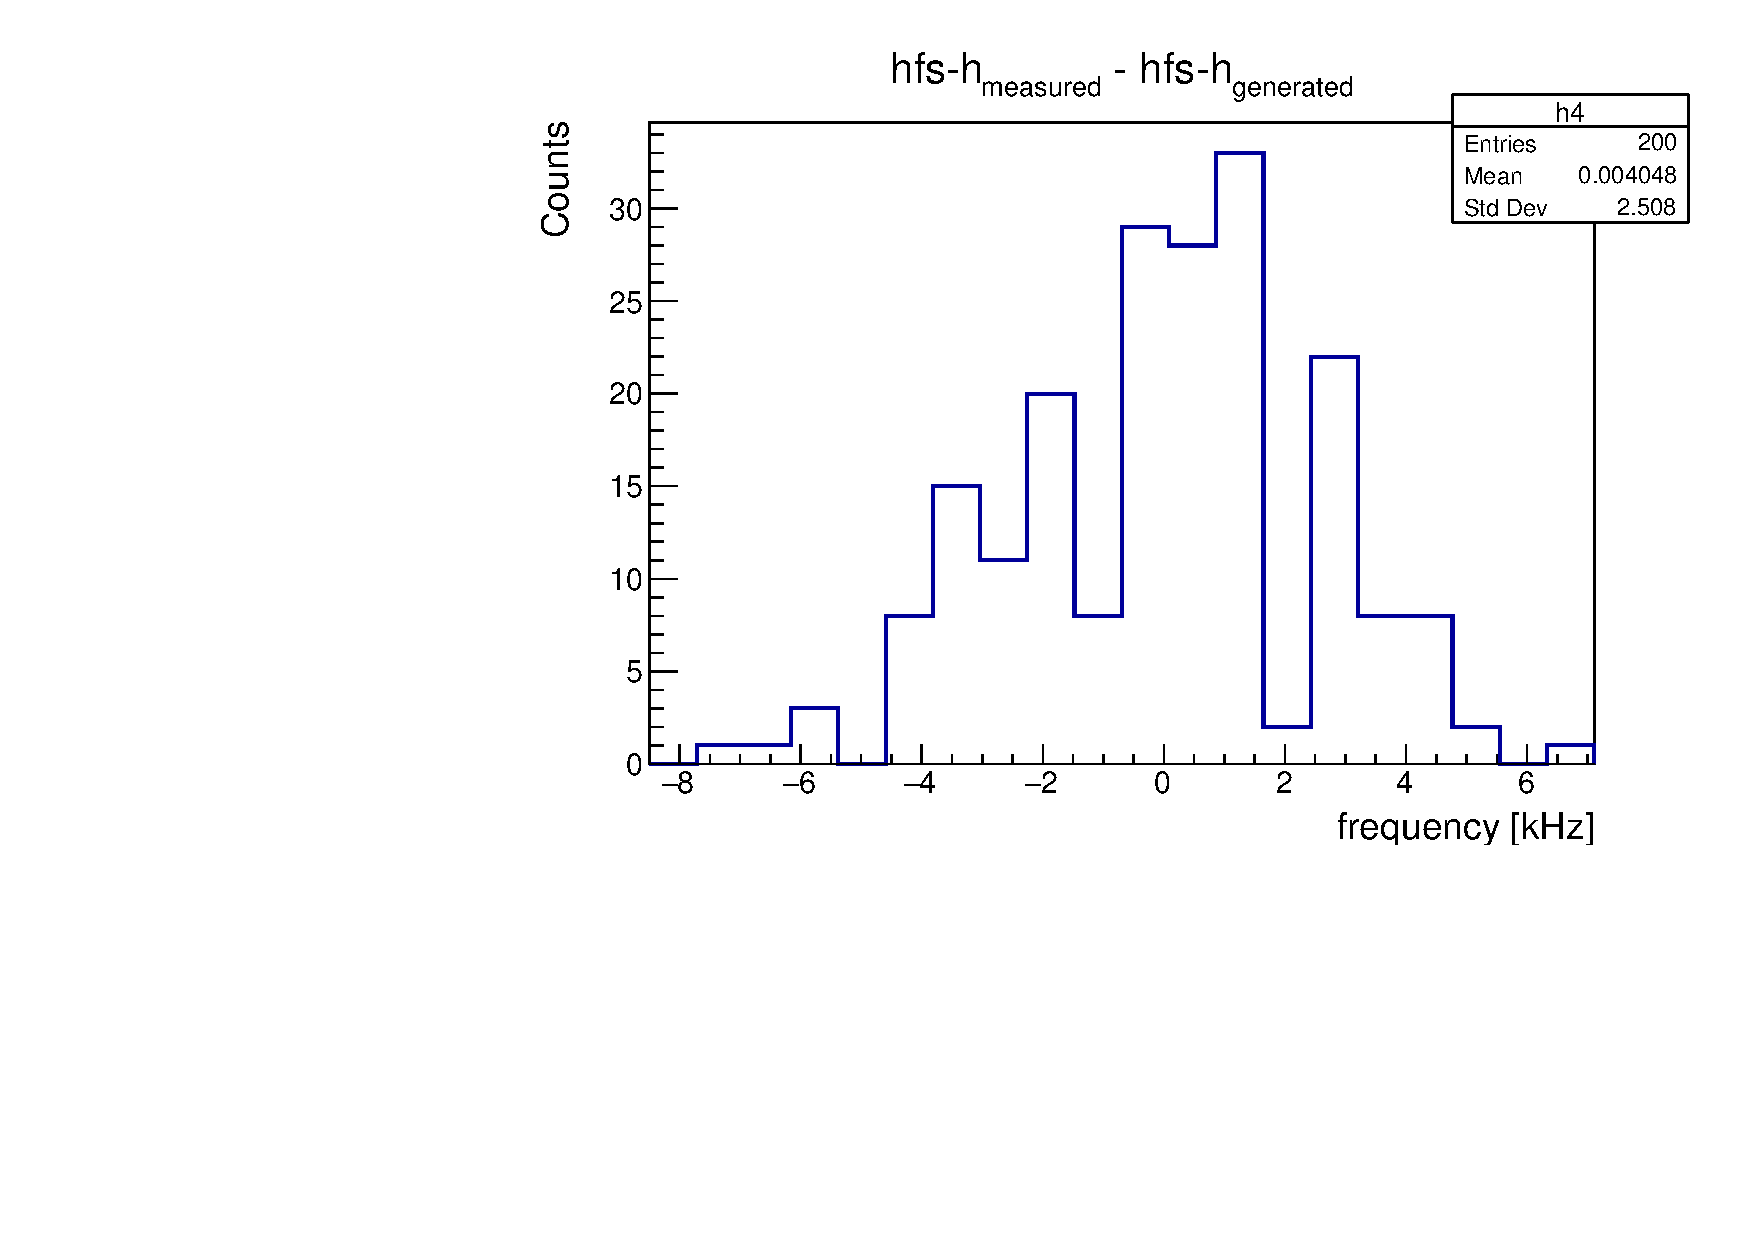
\includegraphics[width = 0.49\textwidth]{significance/4bmuonONresgasOn.pdf}
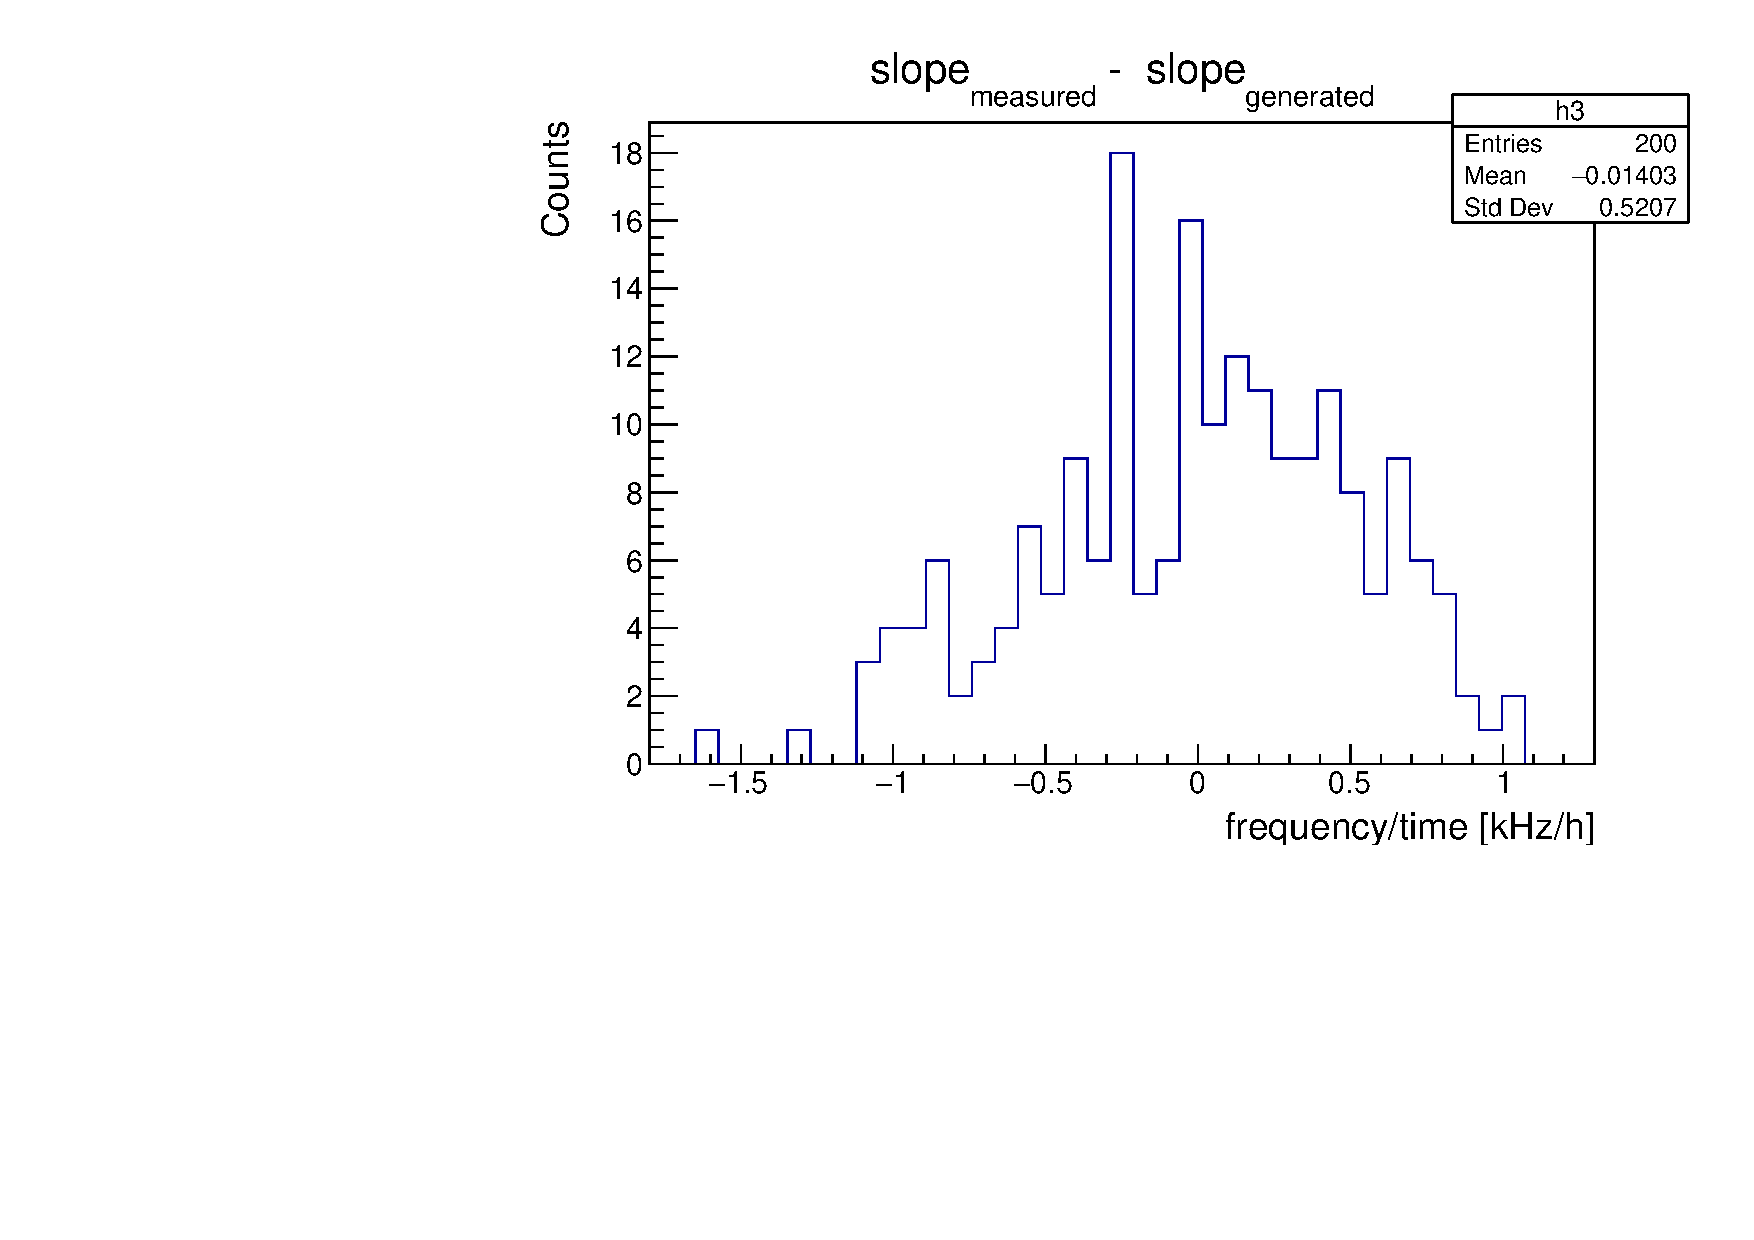
\includegraphics[width = 0.49\textwidth]{significance/4bmuonONresgasOn_slope.pdf}
\caption{4b scenario, on the left the residual between the measured and the Monte Carlo true value hyperfine splitting, on the right the residual between the estimated and the true value of the magnetic drift.}
\end{figure}
\newpage
\subsubsection{Asymmetric rise}

\begin{figure}[hbtp]
\centering
\textbf{FORWARD ALGORITHM 4B SERIE} \vspace{10pt}\\
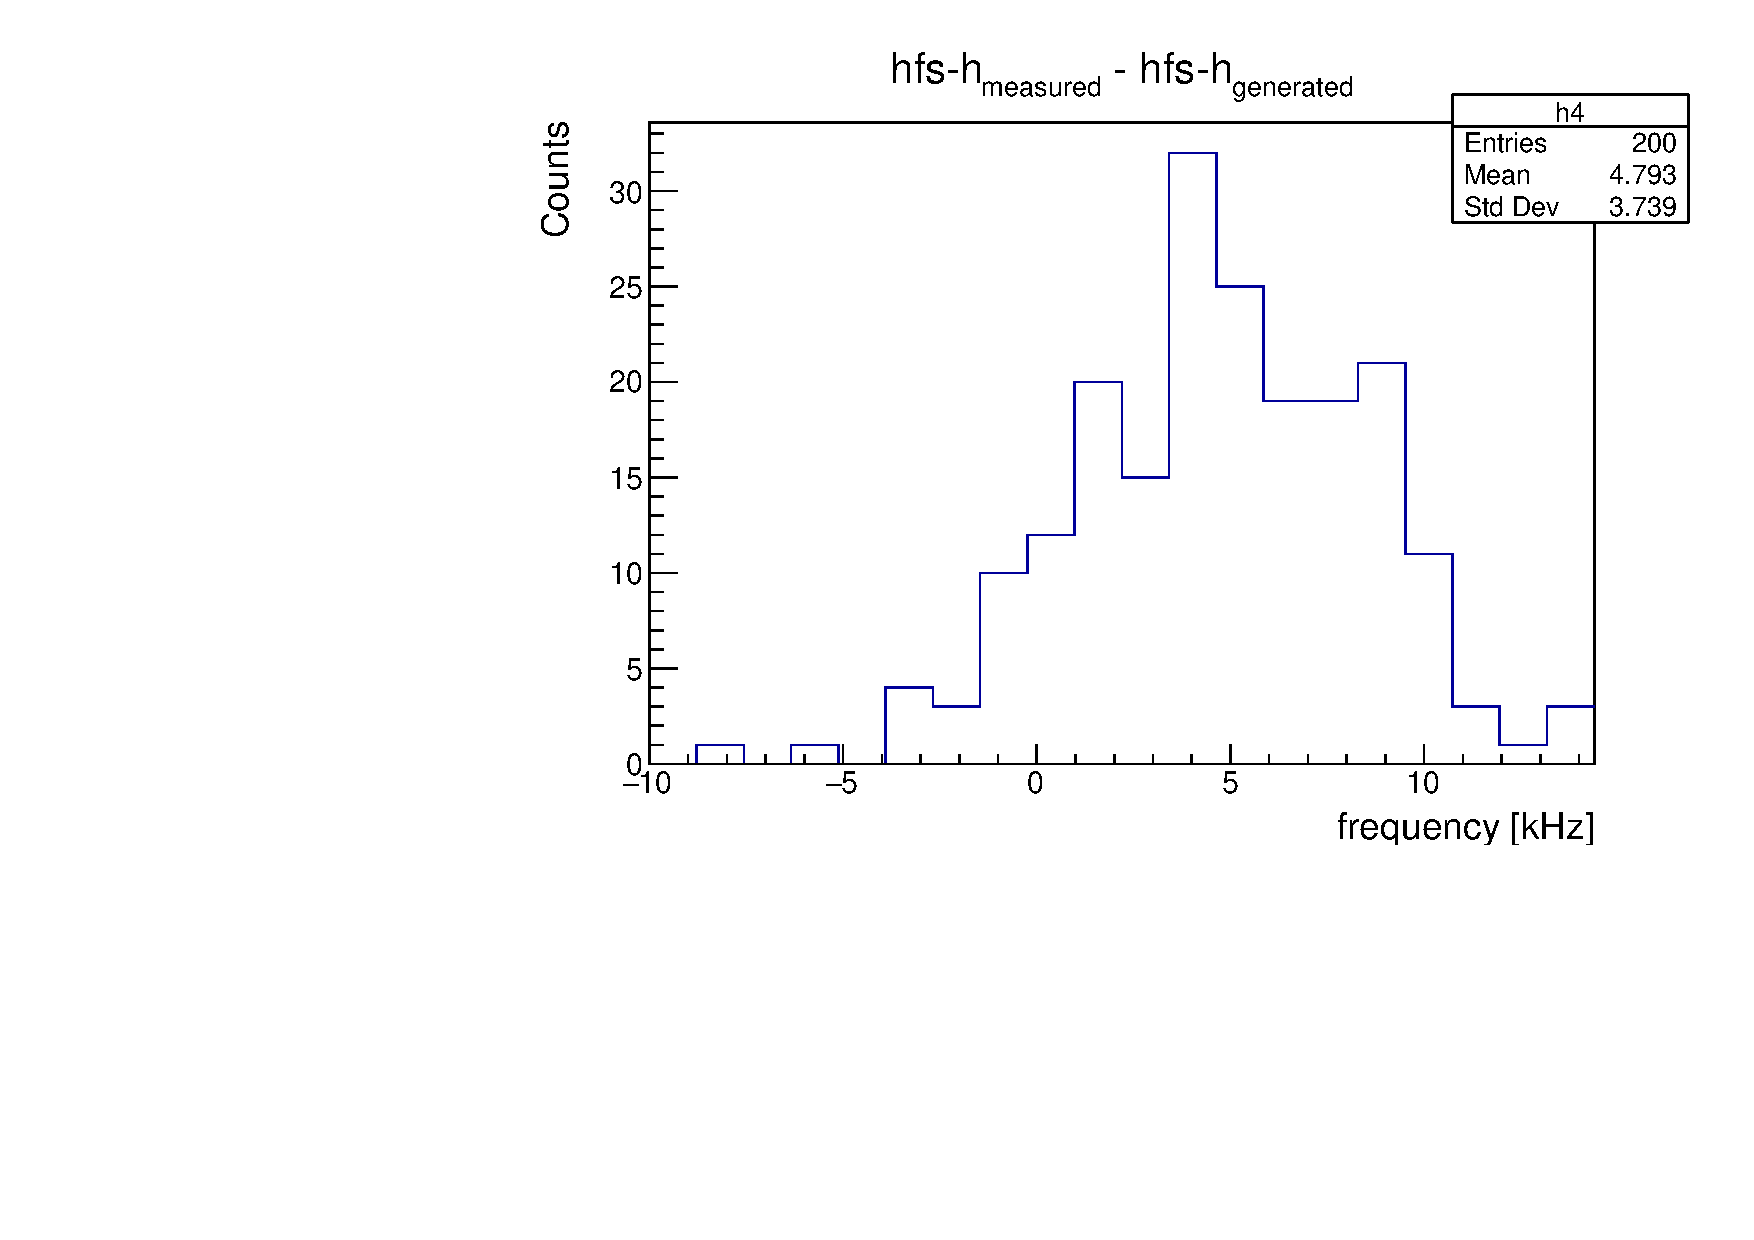
\includegraphics[width = 0.49\textwidth]{forward/4bmuonONrise.pdf}
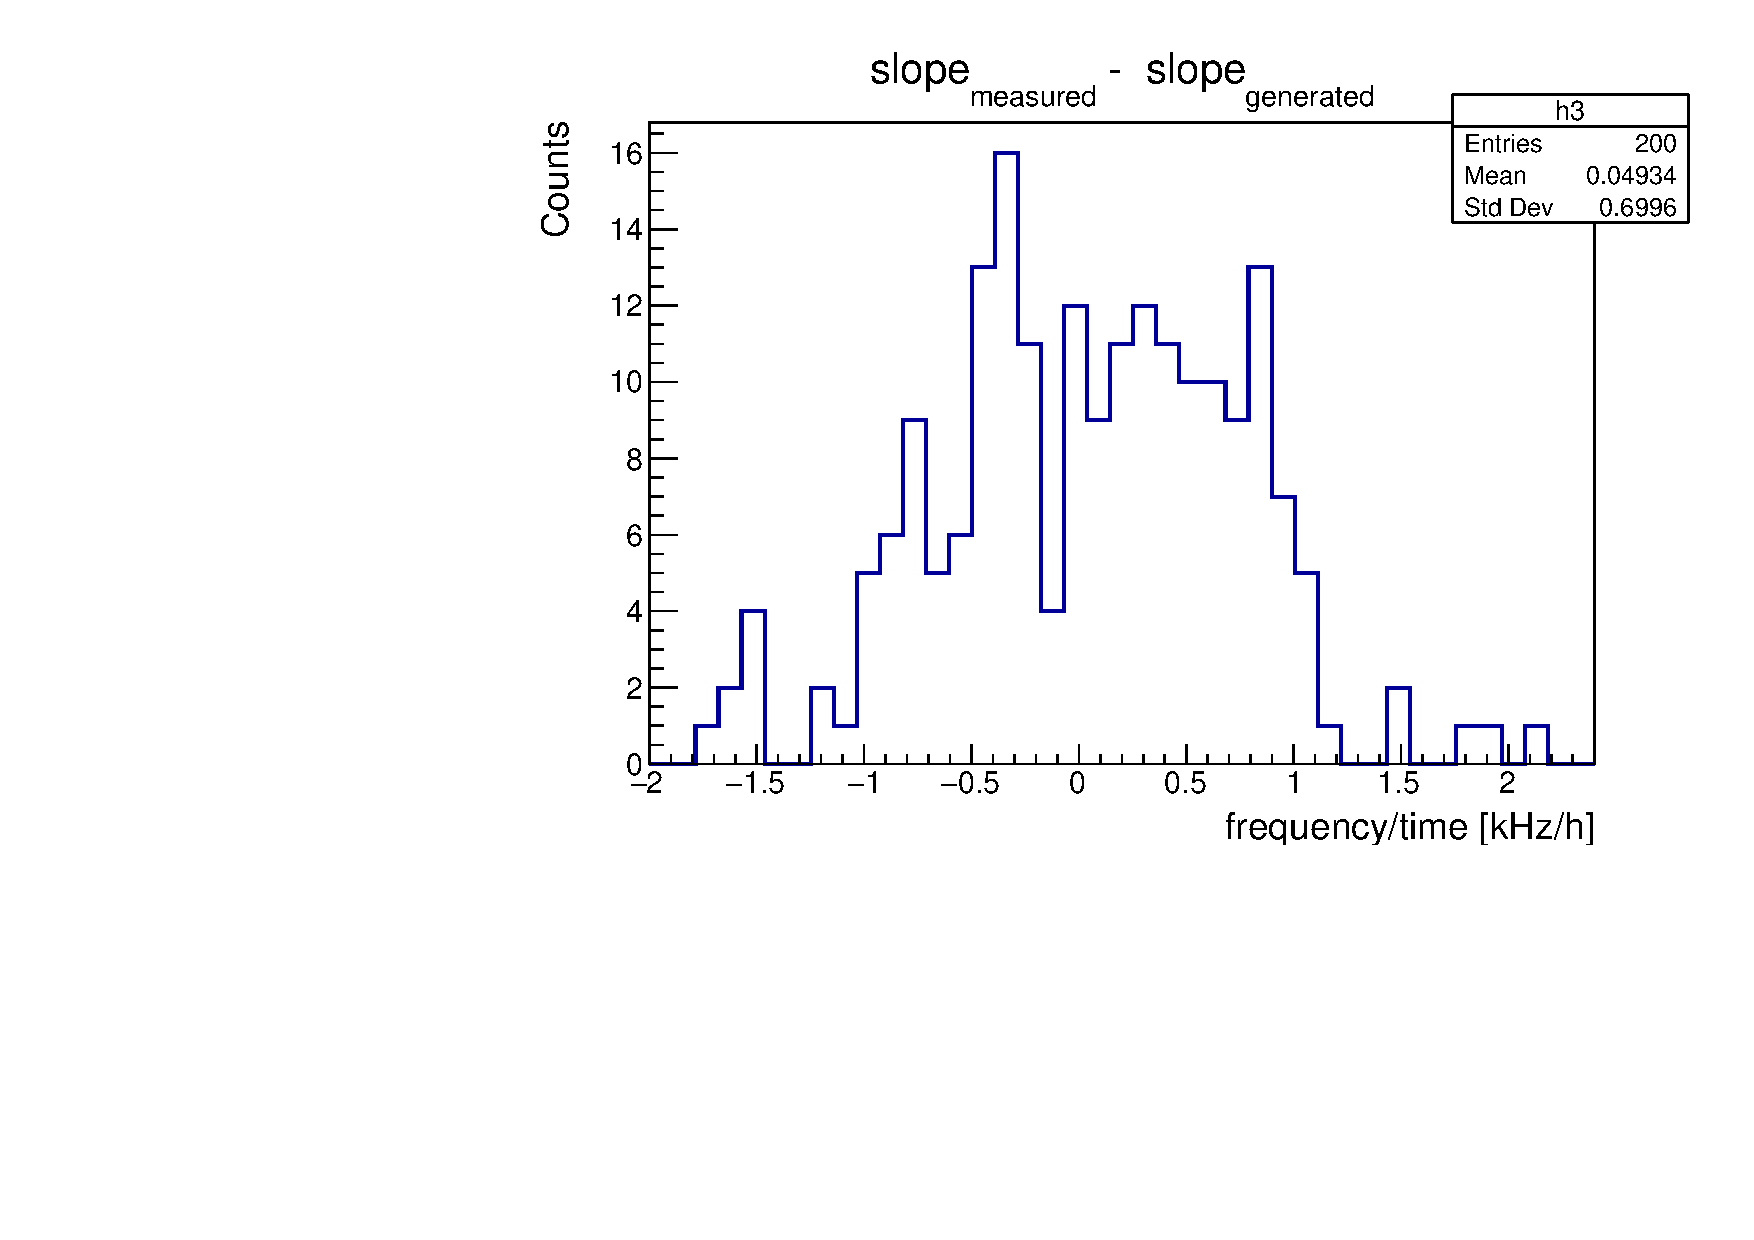
\includegraphics[width = 0.49\textwidth]{forward/4bmuonONrise_slope.pdf}
\caption{4b scenario, on the left the residual between the measured and the Monte Carlo true value hyperfine splitting, on the right the residual between the estimated and the true value of the magnetic drift.}
\end{figure}

\begin{figure}[hbtp]
\centering
\textbf{CONSTANT FRACTION ALGORITHM 4B SERIE} \vspace{10pt}\\
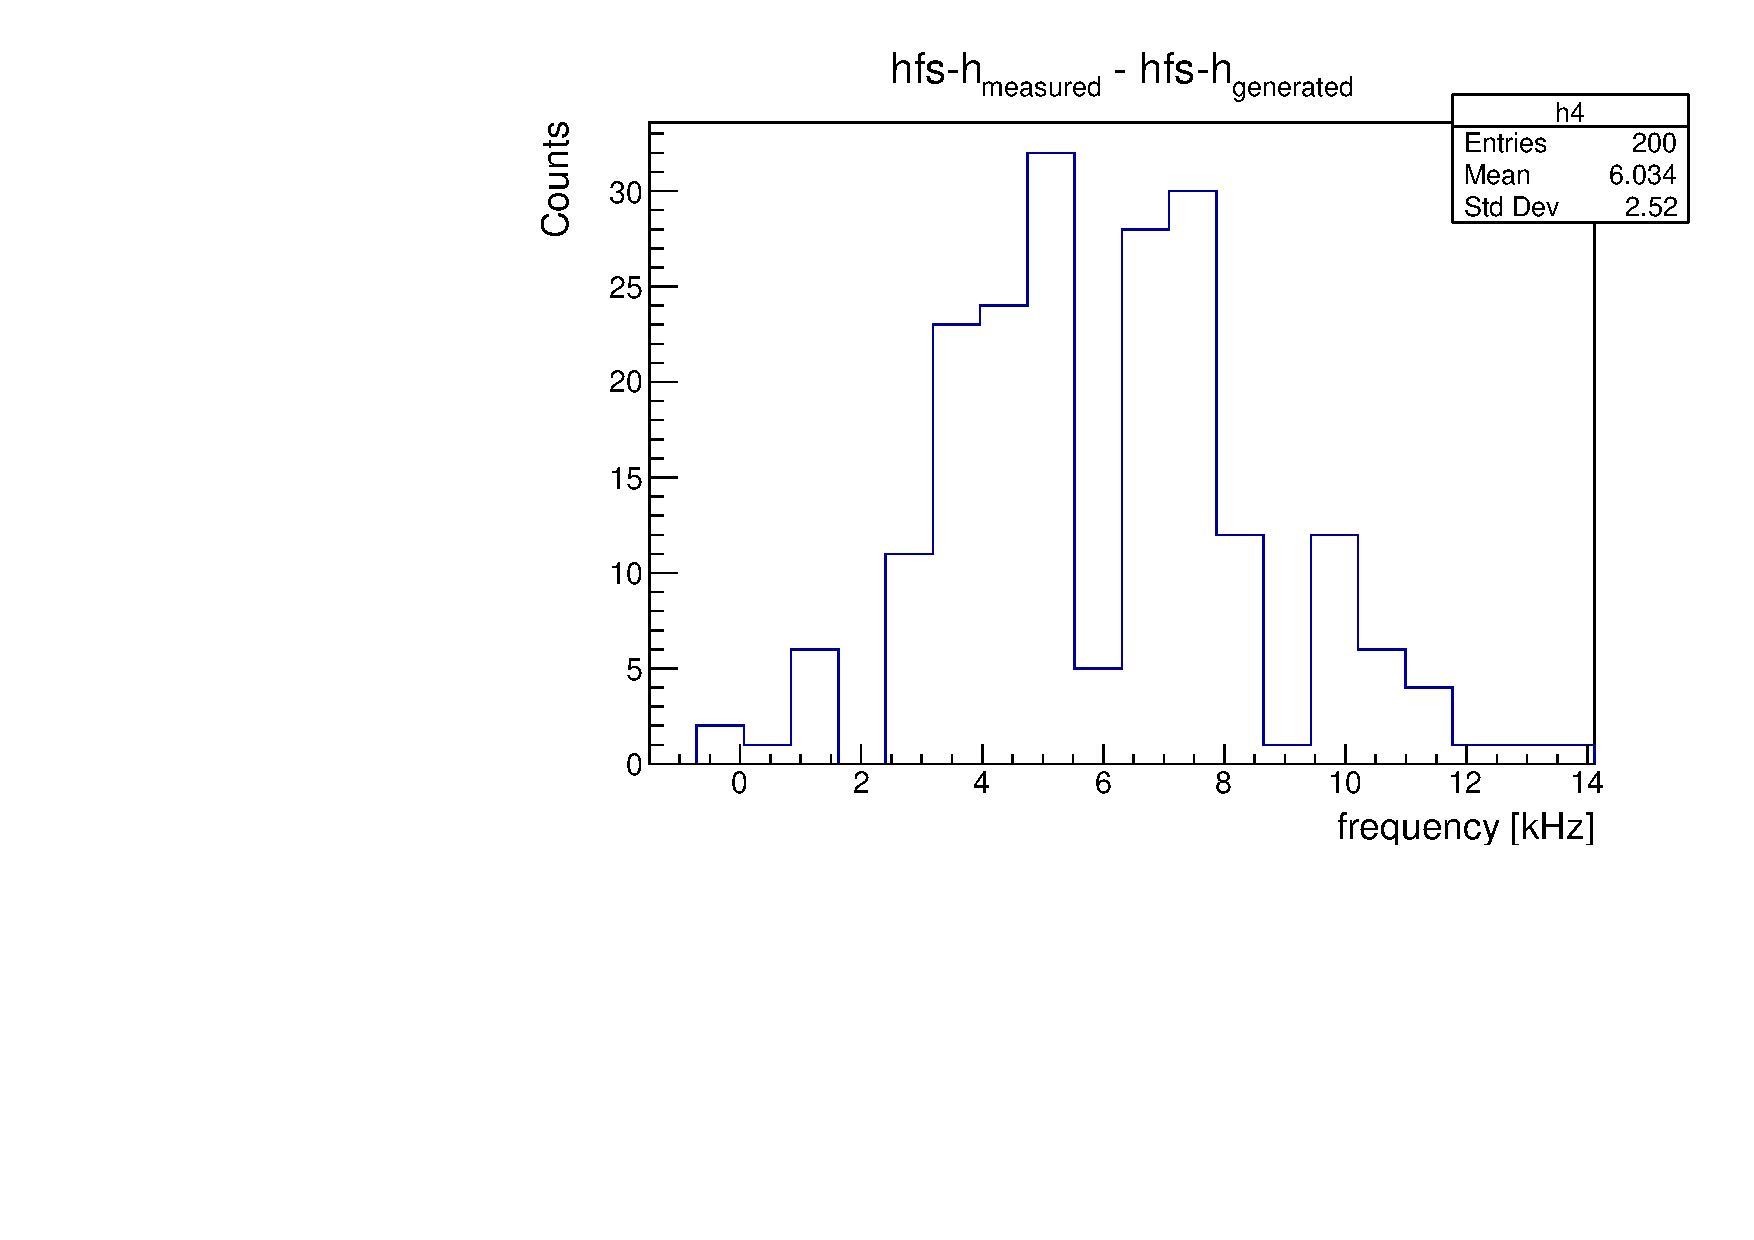
\includegraphics[width = 0.49\textwidth]{constantfraction/4bmuonONrise.pdf}
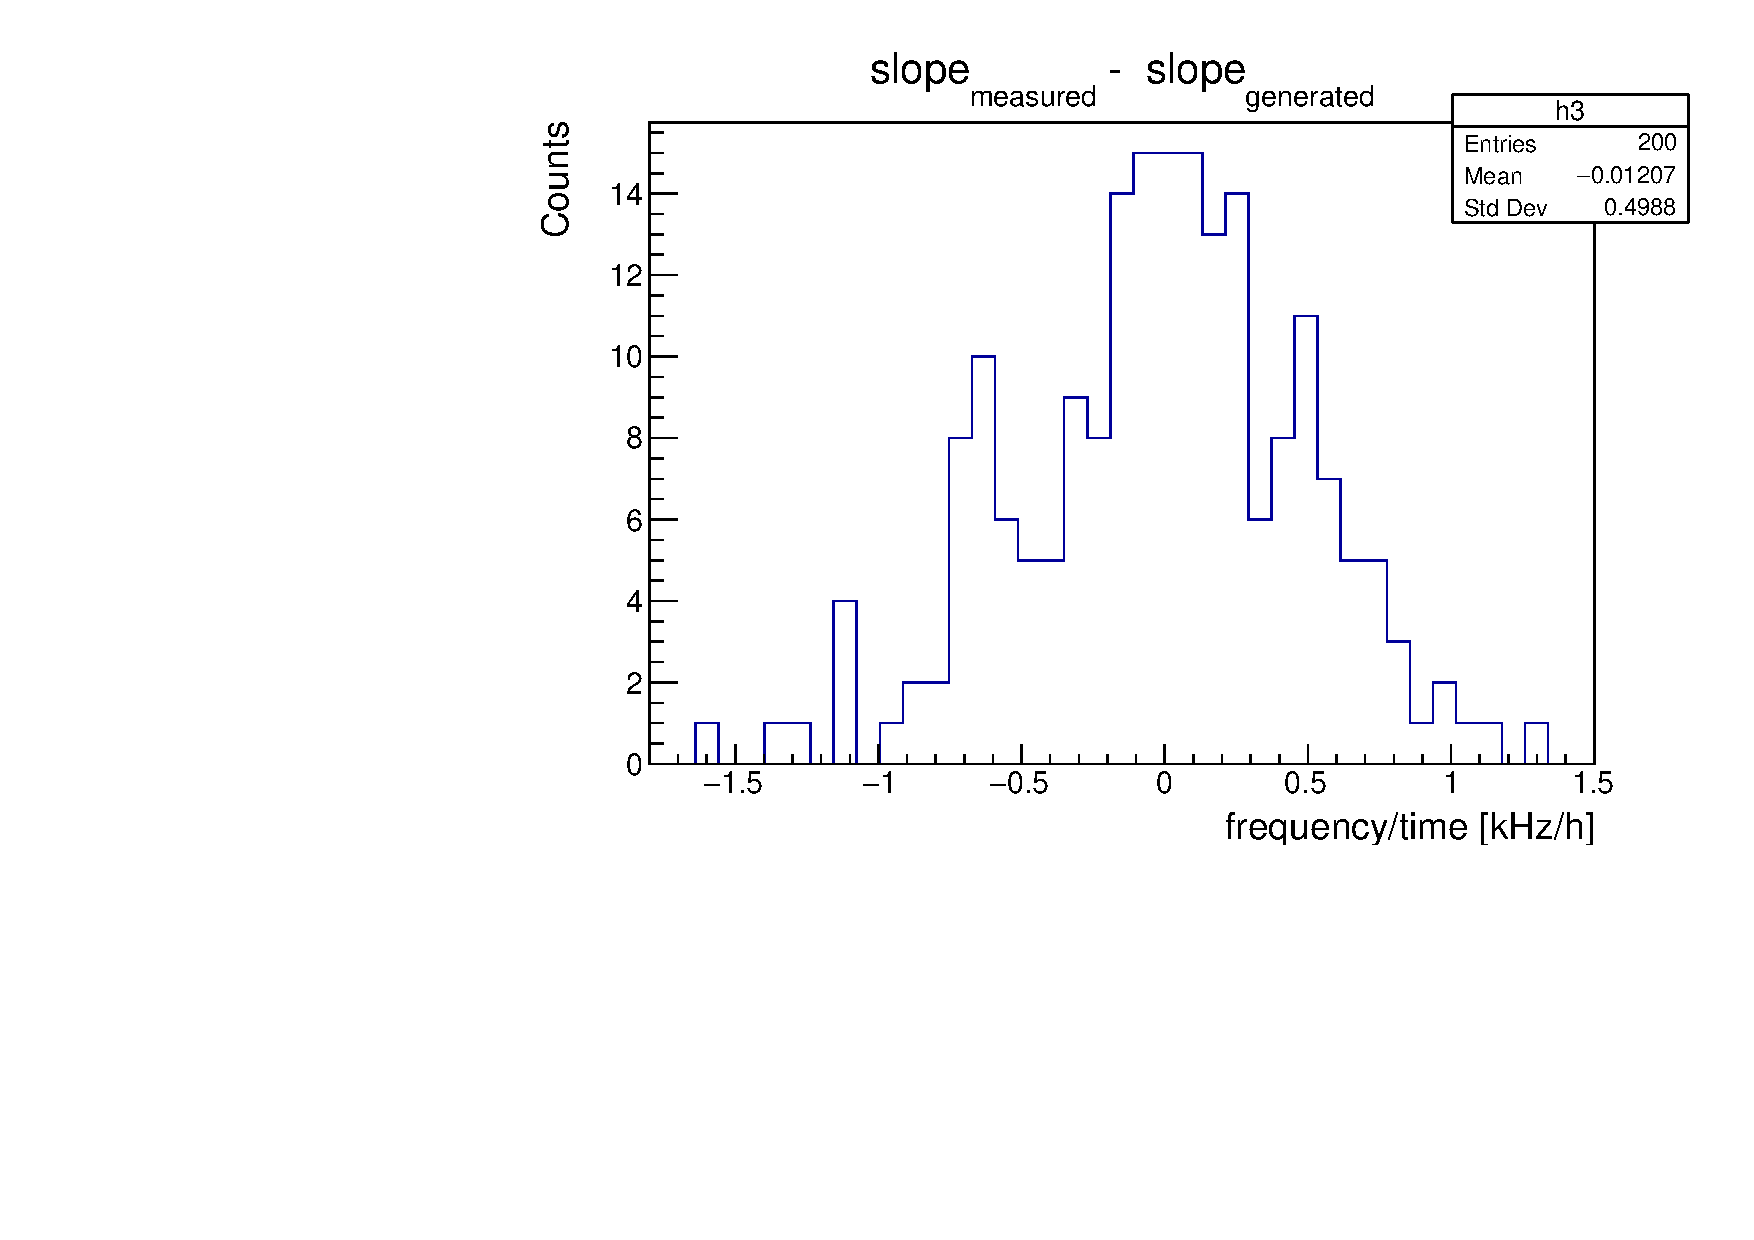
\includegraphics[width = 0.49\textwidth]{constantfraction/4bmuonONrise_slope.pdf}
\caption{4b scenario, on the left the residual between the measured and the Monte Carlo true value hyperfine splitting, on the right the residual between the estimated and the true value of the magnetic drift.}
\end{figure}

\begin{figure}[!hbtp]
\centering
\textbf{SiGNIFICANCE ALGORITHM 4B SERIE} \vspace{10pt}\\
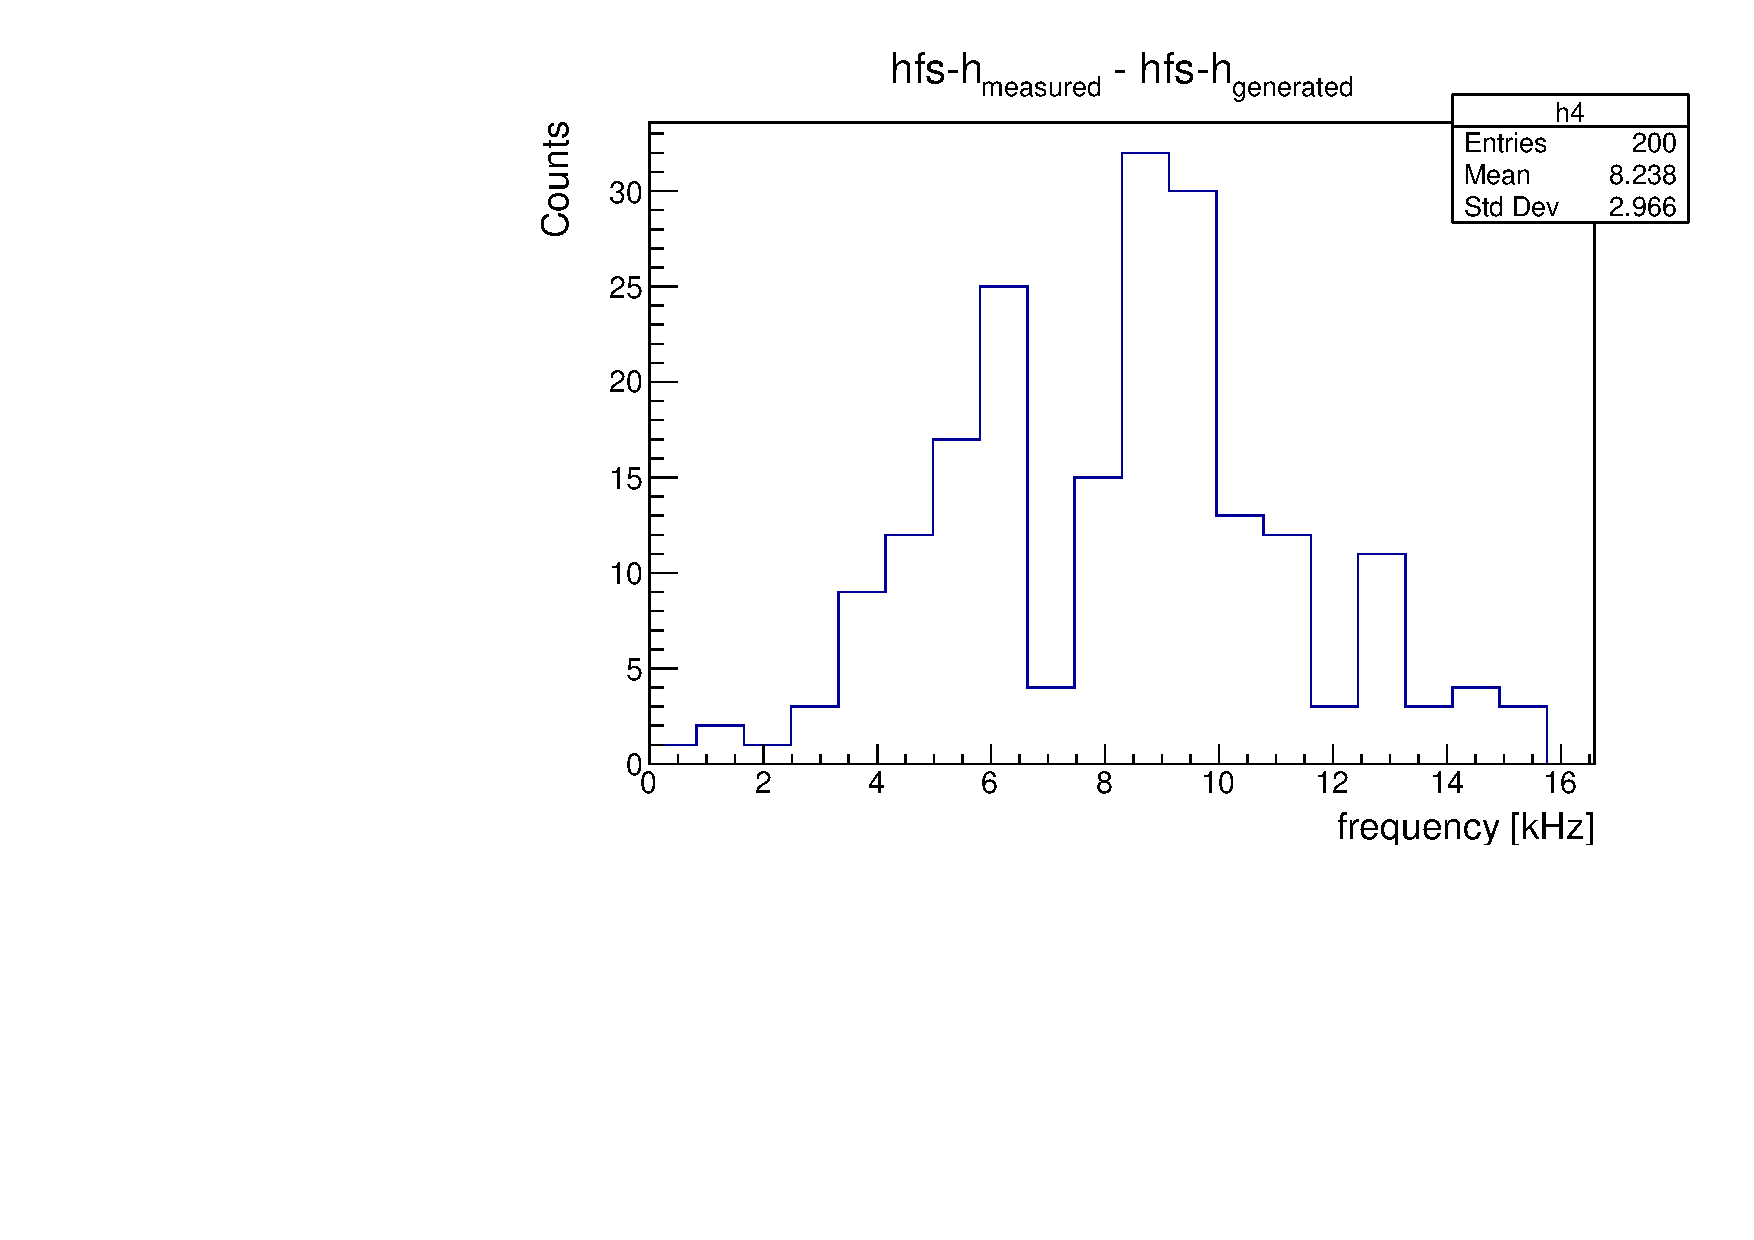
\includegraphics[width = 0.49\textwidth]{significance/4bmuonONrise.pdf}
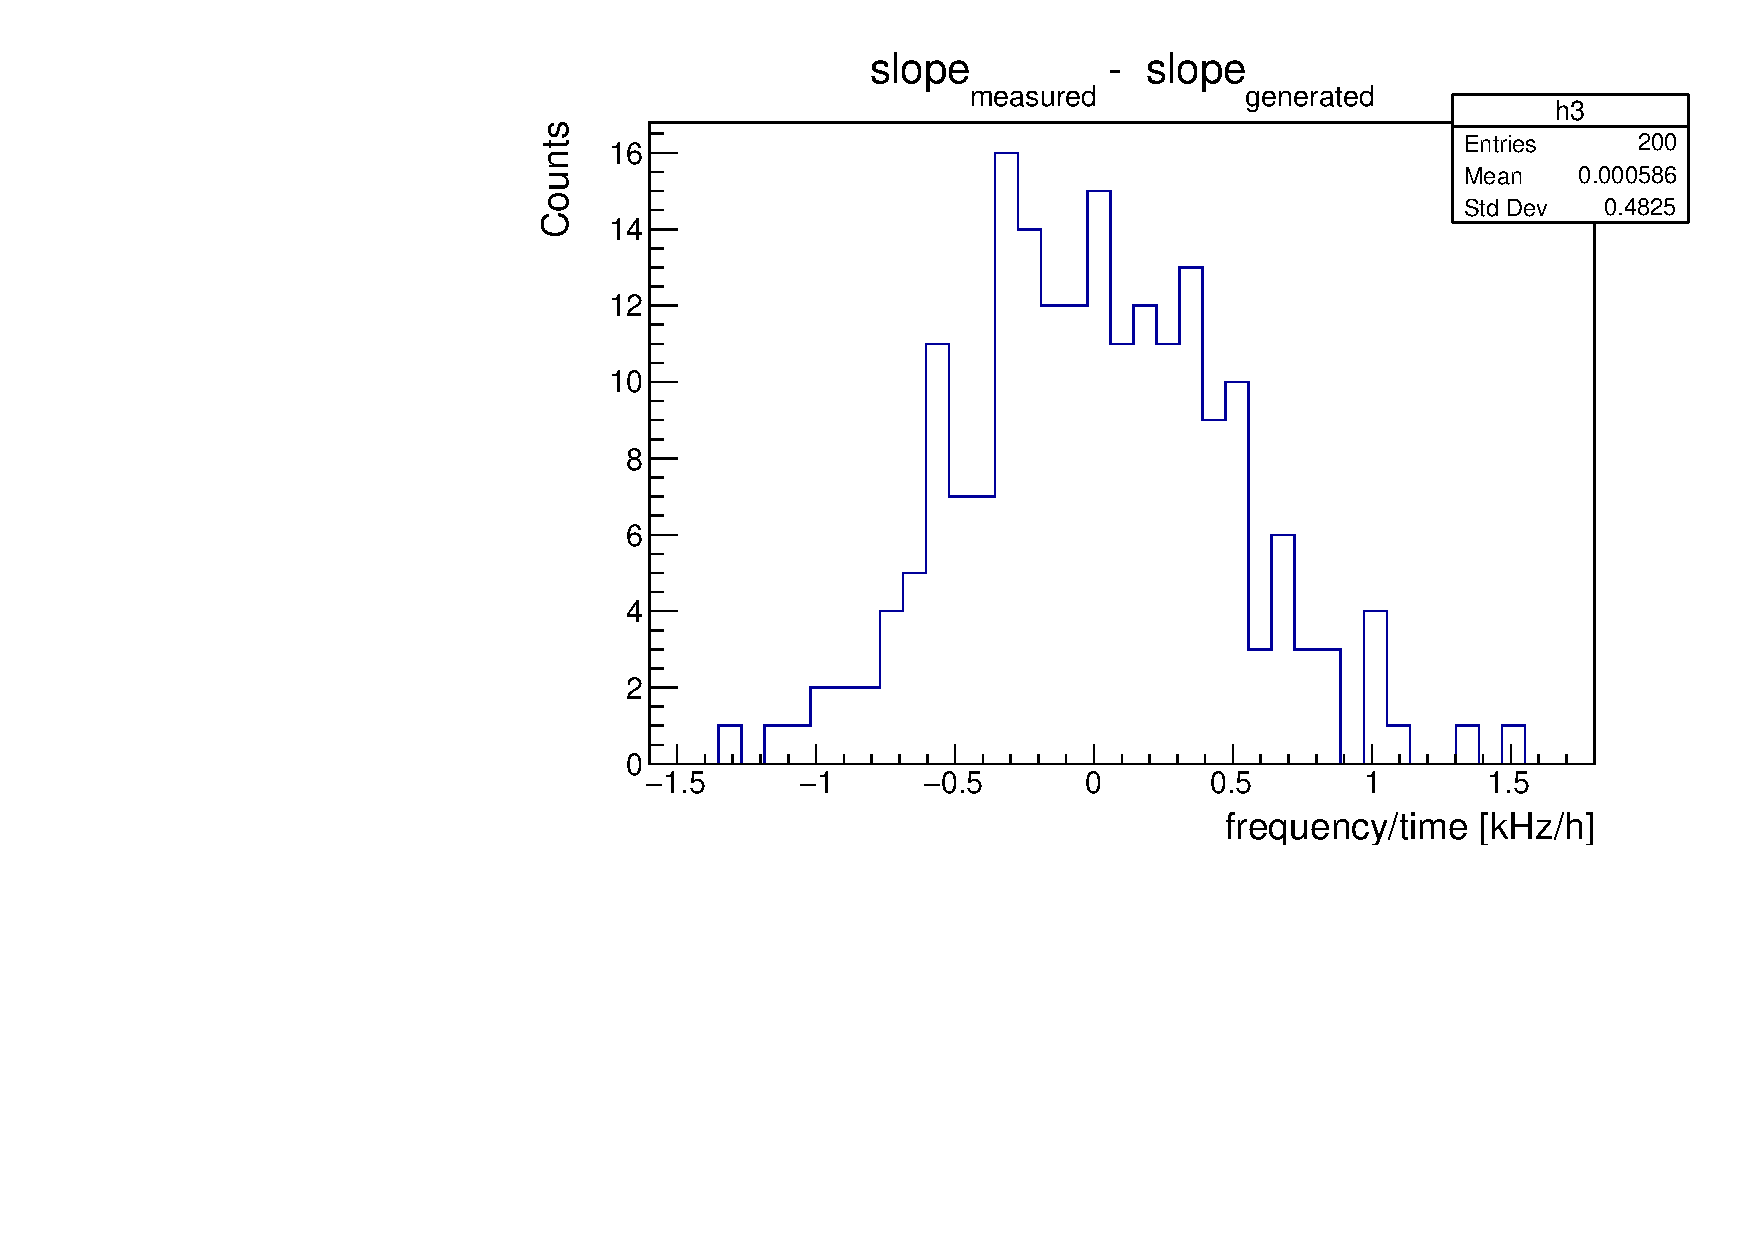
\includegraphics[width = 0.49\textwidth]{significance/4bmuonONrise_slope.pdf}
\caption{4b scenario, on the left the residual between the measured and the Monte Carlo true value hyperfine splitting, on the right the residual between the estimated and the true value of the magnetic drift.}
\end{figure}

\newpage
\subsection{4a scenario}
\subsubsection{Asymmetric background}
\subsubsection{Asymmetric rise}

\newpage
\subsection{Series 3 scenario}
\subsubsection{Asymmetric background}
\subsubsection{Asymmetric rise}

\end{document}